\documentclass[12pt,letter]{article}

%compile with pdflatex:
%:! bibtex %:r
%:! pdflatex -synctex=1 -interaction=nonstopmode --shell-escape %

\usepackage{amsmath}
\usepackage{natbib}
\usepackage{graphicx}
\usepackage{hyperref}
\usepackage{subcaption}
\usepackage{gnuplottex}
\usepackage{caption}
\captionsetup{font={sf,small},labelfont=bf,width=0.95\textwidth}

\usepackage{titlesec}
\titleformat*{\section}{\large\bfseries} %LARGE, Large, large
\titleformat*{\subsection}{\normalsize\bfseries} %LARGE, Large, large
\usepackage{booktabs}
\newcommand{\tabitem}{~~\llap{\textbullet}~~}

\title{Recurrence rate and magma effusion rate for the latest volcanism on Arsia Mons, Mars}
\date{}
\author{}

\usepackage[margin=1in]{geometry}
\usepackage{setspace}
%\doublespacing

\usepackage{lineno}
%\linenumbers


\begin{document}

\maketitle


\section{Introduction}

\citet{greeley1991magma} produced one of the first extrusive magma flux estimates for the surface of Mars and used terrestrial intrusive/extrusive ratios to calculate that $6.5\cdot 10^8$ km$^3$ of magma has been generated on Mars in the past 3.8 Ga. For the most recent 500 Ma, magma production was observed to wane, and only $2.11\cdot 10^6$ km$^3$ of magma was modeled to have erupted \citep{greeley1991magma}. This global extrusive magma flux of 0.004 km$^3$/yr (0.13 m$^3$/s) remains one of few such estimates of magma production. Constraining past and recent magma production and extrusion rates, however, is of vital importance in understanding evolution of the Martian climate \citep[e.g.]{mouginis2008lava,halevy2014episodic}, lithosphere and mantle \citep{grott2013long}, surface \citep{wilson1994mars}, and the ability of Mars to sustain biotic or pre-biotic material over time \citep{scanlon2015volcanism}.

The large volcanic edifices of the Tharsis region have been given a time-averaged magma flux estimate of 0.05 m$^3$/s, with a factor of 3 uncertainty, for an active construction period of 1 Gyr (again with a factor of 3 uncertainty) by \citet{wilson2001evidence}. \citet{wilson2001evidence} further constrained periodic flux under these volcanoes by assuming each of the many summit calderas was formed in association with one stable magma body at depth. By calculating the necessary flux to achieve the magma bodies that could form such calderas, \citet{wilson2001evidence} found that the magma delivery rate to the volcanoes had to persist at 1-10 m$^3$/s for hundreds of thousands to millions of years, followed by orders of magnitude longer periods of quiescence before new large magma bodies could be emplaced. For example, assuming a magma chamber size of 50,000 km$^3$ under the Arsia Mons caldera \citep{wilson2001evidence}, it would take a 10 m$^3$/s magma flux 140 kyr to fill the magma chamber, representing $\sim$3\% of Arsia's total volume in just 0.01\% of a 1 Gyr constructional period.

We seek to estimate both the recurrence rate of volcanism and the extrusive magma delivery rate for the most recent volcanic unit on Arsia Mons---a patchwork of lava flows and 29 associated volcanic vents within the volcano caldera. To constrain these values, absolute ages and associated age uncertainty of each flow have been modeled using the size-frequency distribution of observed craters, relative ages between flows have been determined using superposition relationships, and volumes have been modeled using Mars Orbiter Laser Altimeter (MOLA) data \citep{smith2003mars}. Crater-retention age models and stratigraphic relations are integrated in a Volcanic Event Recurrence Rate Model (VERRM) to better characterize event age uncertainty and estimate recurrence rate throughout the period of time during which these lavas were emplaced.

\begin{figure}
\centering
\includegraphics[width=0.5\linewidth]{figures/fig_catalog}
\caption{The Tharsis Volcanic Province of Mars. Each black dot represents one small volcanic vent in a Tharsis-wide catalog. Within Arsia Mons (bottom left), 29 vents have been identified. The color relief basemap is MOLA topography.}
\label{fig_locatormap}
\end{figure}

\section{Geologic Background of Arsia Mons}

Arsia Mons is a major shield volcano on Mars and a member of the Tharsis Montes (Figure \ref{fig_locatormap}). With a diameter of over 300 km and slopes of 5$^{\circ}$ \citep{plescia2004morphometric}, the surface of Arsia contains lava flows, which served as the primary construction material of the shield \citep{mouginis2008lava}, prodigious ash deposits \citep{mouginis2002prodigious}, and glacial deposits \citep{head2003cold} emplaced under both cold- and warm-based glacial conditions \citep{scanlon2015volcanism}. At the summit of Arsia is a single collapse caldera measuring $\sim$4000 km$^3$ in volume \citep{wilson2001evidence}. Within this 110 km wide caldera, a linear cluster of secondary shield volcanoes comprise one of the youngest geologic units in the Arsia region \citep{carr1977some,scott1995geologic}. No craters larger than 1 km exist within the caldera and several detailed crater retention studies with different image datasets have independently produced 130 Ma as a single age estimate of the entire caldera floor \citep{neukum2004recent,werner2009global,robbins2011volcanic}.

Through Mariner 9 and Viking Orbiter images of the Tharsis region, \citet{crumpler1978structural} determined that of the three Tharsis Montes, Arsia Mons is the most structurally evolved shield volcano. This conclusion was backed up by \citet{bleacher2007tharsis} with extensive mapping using HRSC and THEMIS. \citet{bleacher2007tharsis} suggested that the northward trending structural complexity of the Tharsis Montes might indicate a migrating magma source along the axis of the three volcanoes, similar to a Tharsis plume model by \citet{mege1996plume}. If such a migrating magma source did exist, then magma production at Arsia would have waned, decreasing the amount of melt available for continued summit volcanism.

\begin{figure}
\centering
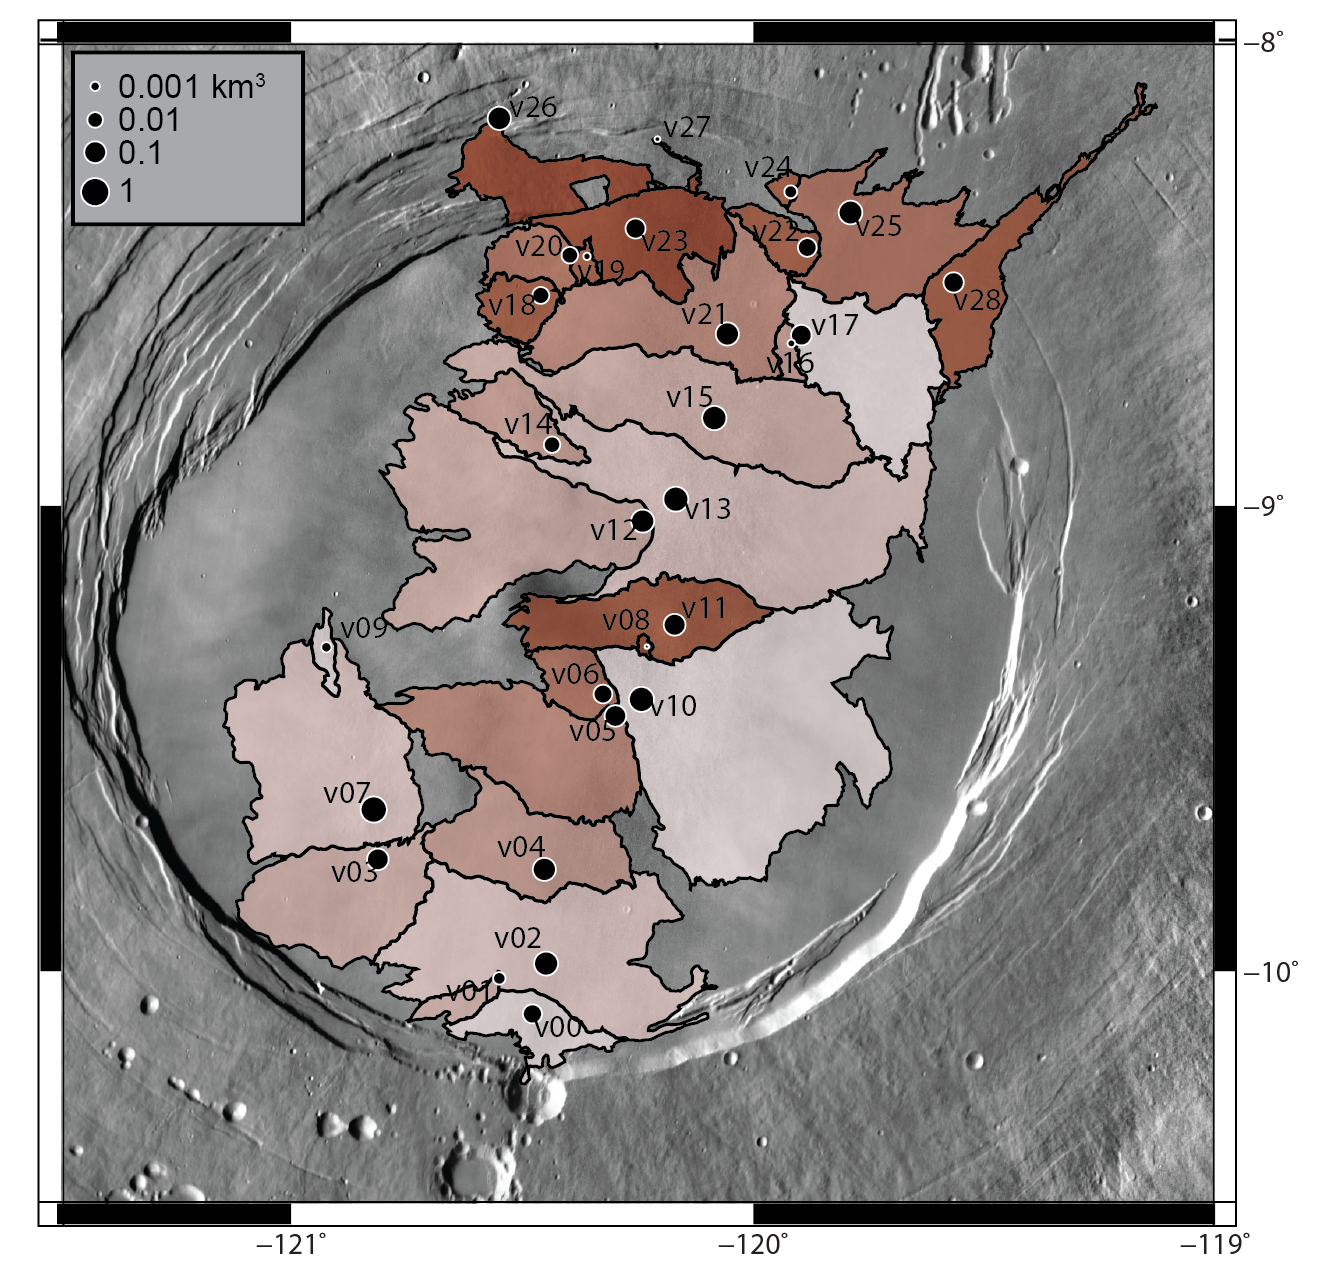
\includegraphics[width=0.7\linewidth]{figures/vent_map-01}
\caption{Mapped lava flows in the vent field. Circles are placed at the 29 vent locations and are sized according to volume. Lighter colored flows are higher stratigraphically than darker colored flows (See Figure \ref{fig_stratweb}).}
\label{fig_lavamap}
\end{figure}

On the flank of Arsia Mons, \citet{mouginis2008lava} identified $>$1000 layered units in a graben, which were interpreted to be lava flows. Using MOLA data, they were able to estimate the height of the graben wall, enabling the estimation of layer thicknesses between 10-80 m, with most being $>$30 m. As no unique and laterally extensive layers were observed in the stack of $<$2 km wide layers, \citet{mouginis2008lava} concluded that no major glacial events were emplaced between the deposition of these layers, perhaps indicating relatively rapid emplacement of 885 m of lava. By instead assuming constant activity of Arsia Mons for either 2 or 3 billion years, \citet{mouginis2008lava} estimated that the stack could have been emplaced over 290 or 435 million years, respectively. 

\subsection{Other recent volcanism in the Tharsis Region}

Outside of Arsia, several volcanic events and trends in the Amazonian Period ($<$3~Ga) have been identified. On Olympus Mons, the latest flank lava flows appear to have transitioned from long tube-fed flows to shorter, channel-fed flows, suggesting that magma flux per flow emplacement event waned over the late Amazonian \citep{bleacher2007olympus}. \citet{bleacher2007olympus} concluded that this might be evidence of a larger waning of activity at Olympus and might also signal a transition from a deep mantle source of volcanism to shallower sources, based on long-term volcanic patterns observed at the Hawaiian volcanic chain. These observations might be consistent with the \citet{wilson2001evidence} model that most of the history of these volcanoes is spent dormant after hyper-active edifice building episodes wane and end.

Recent volcanism elsewhere in Tharsis has occurred in a more distributed fashion \citep{hauber2011very}, including a lava field filling the southeast ``moat'' of Olympus Mons \citep{chadwick2015late}. \citet{chadwick2015late} identified lava flows at the base of Olympus emplaced between 64-210 Ma, similar in time to previous age estimates of the study area in this paper ($\sim$130~Ma). The emplacement direction of these lavas are systematically offset from the current downward direction, due to recent subsidence of Olympus Mons. This might provide evidence contrart to he findings of \citet{bleacher2007olympus}, as \citet{chadwick2015late} estimate that the magma required to be injected into Olympus Mons the past 200 Myr in order to cause this subsidence might be 10$^5$-10$^6$ km$^3$.

\section{Methods}

\subsection{Unit and stratigraphic mapping}

\begin{figure}[h]
\centering
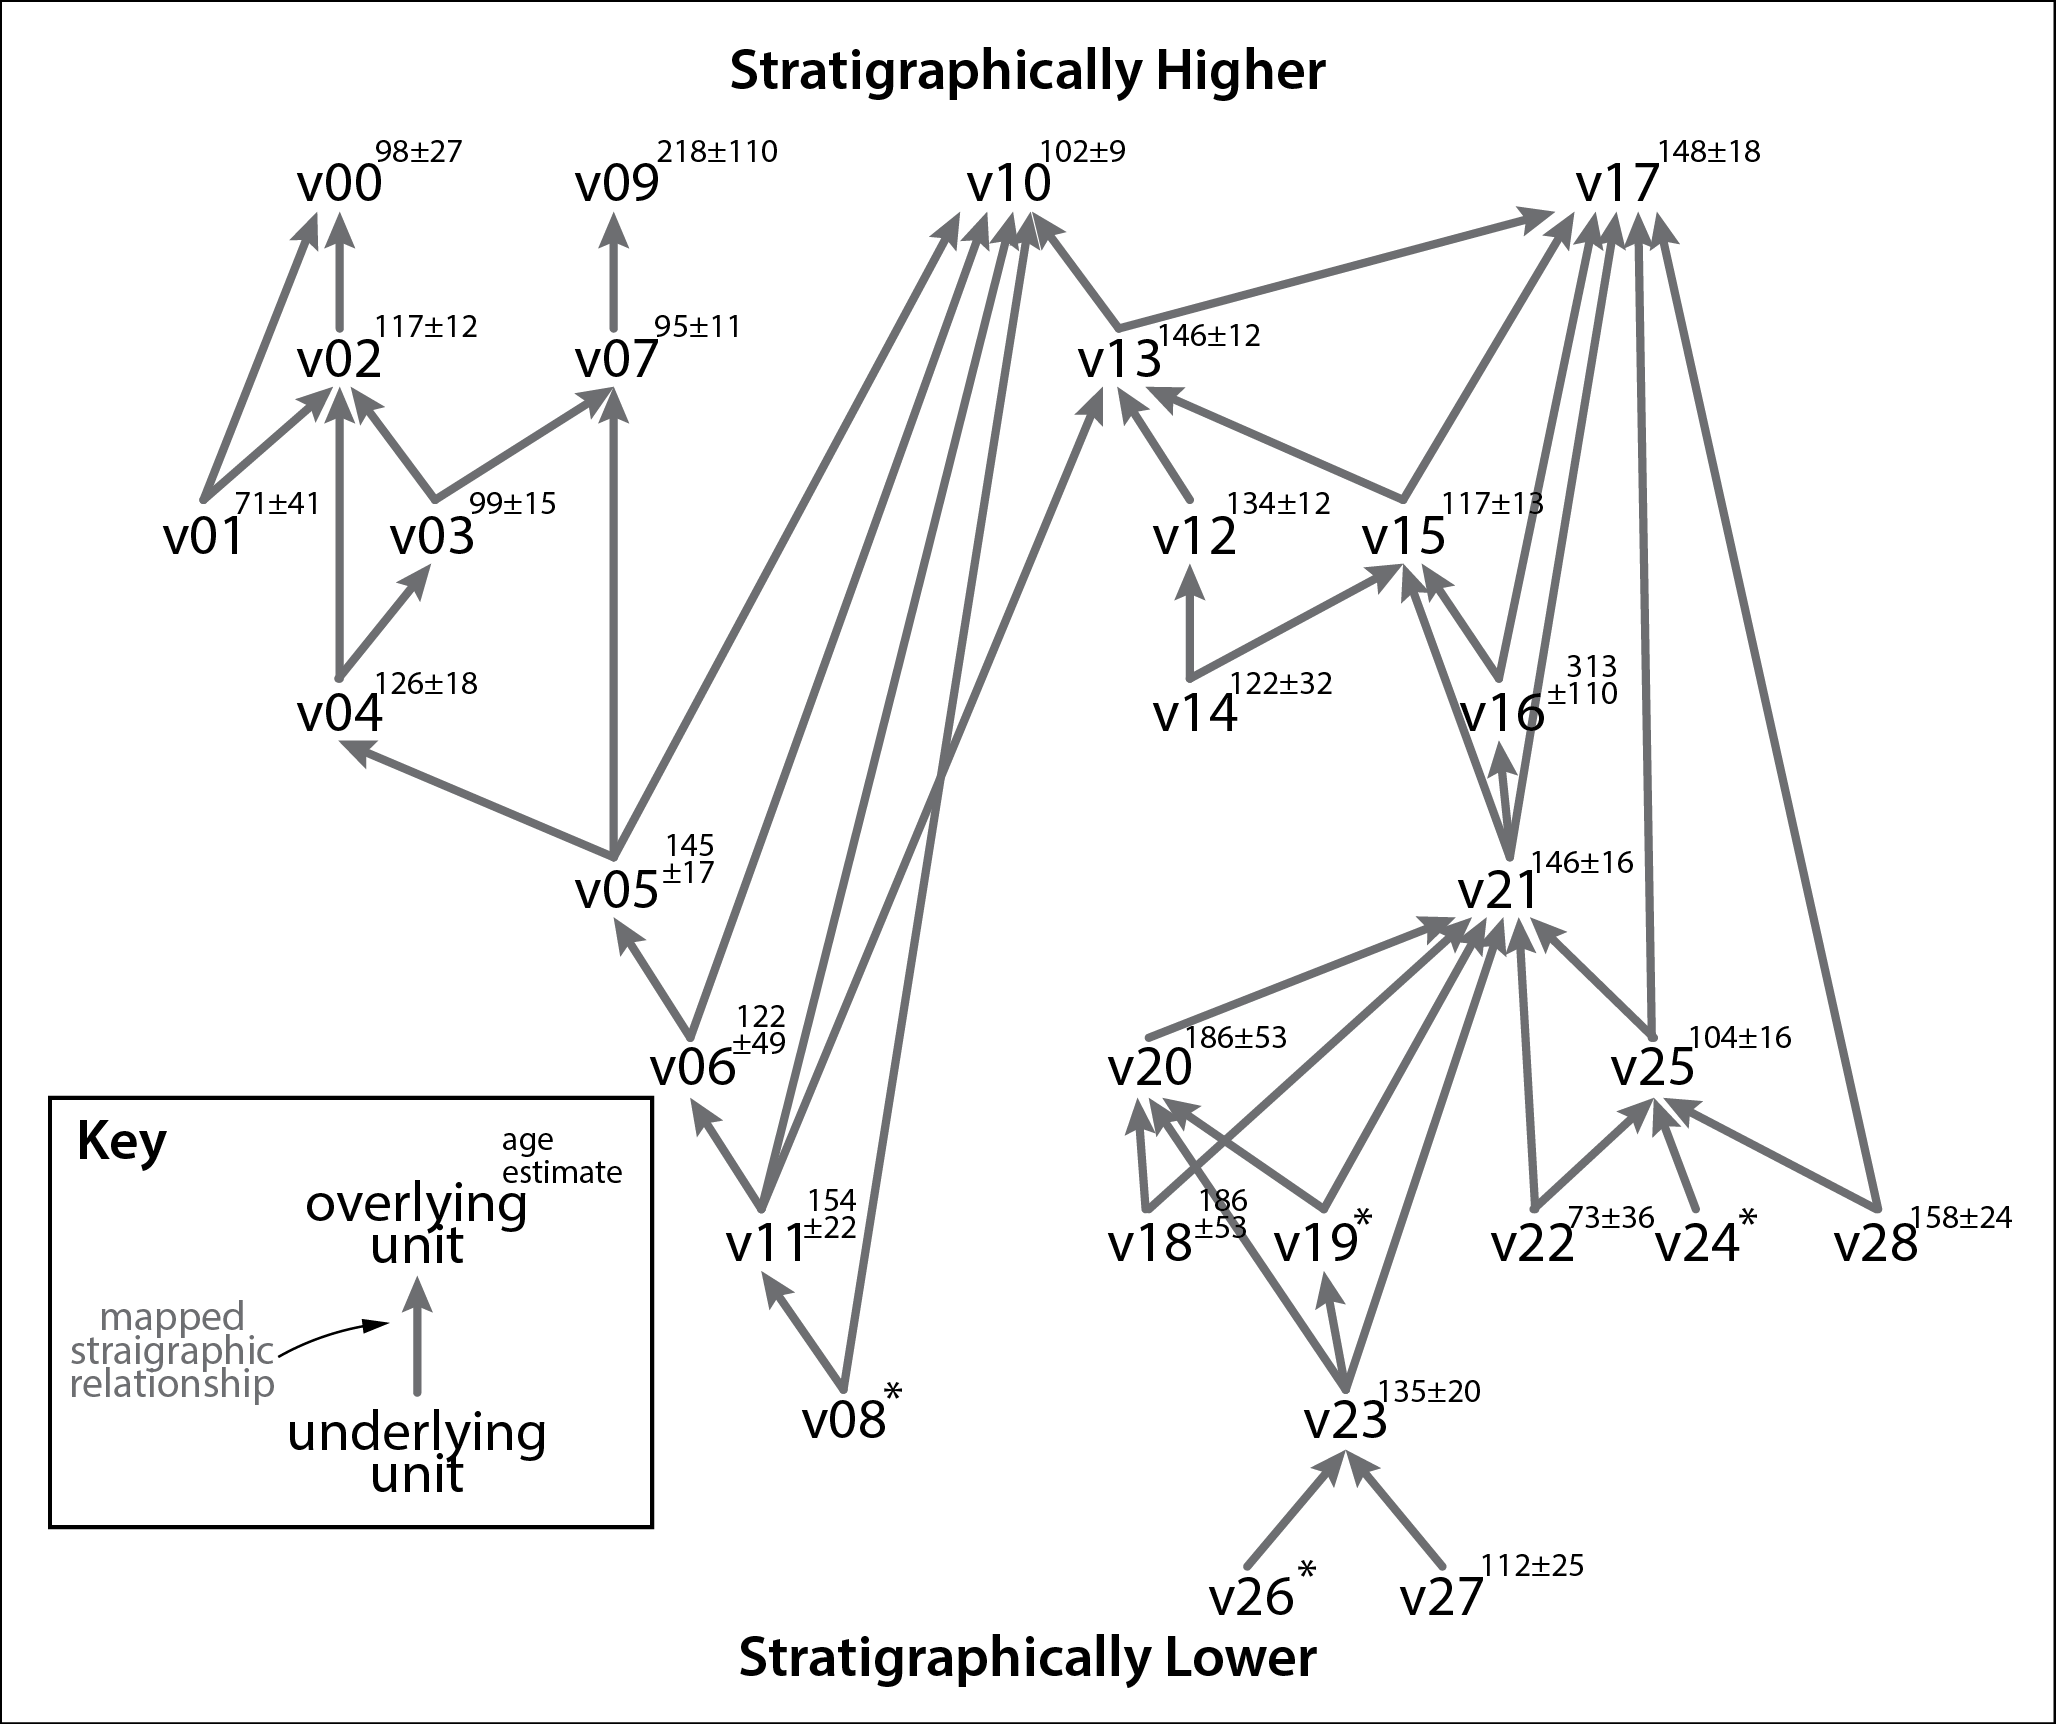
\includegraphics[width=0.7\linewidth]{figures/stratigraphy_web_300dpi.png}
\caption{A directed graph of stratigraphic relationships within the Arsia Mons Caldera. Graphically higher flows (e.g. v00) are higher stratigraphically and directly overlay flows that have connecting lines to them. Each line is one mapped stratigraphic relationship connecting an overlying flow and an adjacent underlying flow. Age estimates from craterstats2 are given in superscript; * symbols indicate no age was estimated due to a lack of craters with D$\ge$100~m.}
\label{fig_stratweb}
\end{figure}

The 29 mapped volcanic vents within the caldera each have lava flows emanating from them that form positive topographic features over the surrounding terrain. Flows corresponding to each vent have been mapped in ArcGIS 10.2 with georeferenced Context Imager (CTX) photographs \citep{malin2007context} serving as a 6-m resolution basemap (Figure \ref{fig_lavamap}). Flows are mapped in association with an observed vent where flows can be unambiguously traced directly back to the vent using flow features. Some lava flows on the eastern and western margins of the caldera appear to flow away from the caldera center and might have been created during an event that formed any of the observed vents; however, because they are covered in subsequent flows and are separated from their parent vent by at least one flow front, they cannot be traced to a vent and are not included in our catalog.

Mapped flows which abut each other have an inherent superposition relationship. Using available CTX images, these relationships are documented for all neighboring flows by identifying features such as 1) diverted flows around pre-existing topography, 2) infilling of graben or volcanic vents, and 3) continuous flow features suddenly vanishing under overlying flows. Superposition relationships are graphed according to stratigraphic height in Figure \ref{fig_stratweb}.

\subsection{Crater retention age modeling}

Mapped units within the caldera (29 lava flow units and 1 ``undifferentiated lavas'' unit) have been assigned model ages based on the distribution of impact craters within their boundaries. \citet{robbins2011volcanic} previously found that, in the Arsia Mons caldera, crater frequency decreases for craters with diameters (D) of $\le$ 93~m, due to dust cover. \citet{robbins2011volcanic} also hypothesized that a background population of secondary craters in this area might contaminate the crater distribution at D $<$ 130 m. We have counted all craters in the caldera with D $\ge$ 100 m to avoid both of these systematic biases. Four lava flows have an exposed area smaller than 15 km$^2$ and an insignificant number of craters larger than 100~m were found on their surfaces (10 or fewer), so no crater age date was determined. The diameter and location of craters were mapped in ArcGIS~10.2 using a basemap of CTX images.

Modeled ages based on a impact production function, which is a model of the relative production rate of different impact crater sizes, and a chronology function, which models the change of impact frequency with time. Ages were modeled in the Craterstats2 software \citep{michael2013planetary}. For each mapped unit, craters are separated by diameter into bins of minimum diameter $2d$~km where $d$ increments by 0.5 between each bin, following the Hartmann 2004 iteration Production Function \citep{hartmann2005martian}. Ages are modeled based on this Production Function and the \citet{michael2013planetary} Chronology Function. Uncertainty of crater frequency in each bin is defined as $\sqrt{N}/S$, where $N$ is the number of craters and $S$ is the area of the mapped unit. The cumulative crater-size frequency distribution (and associated uncertainty) is assembled from each $2d$ km bin and is used to model a best fit age (see Figure \ref{fig_craterct}. Ages and uncertainties for each mapped unit are reported in Ma.

\subsection{Volume estimation}\label{sec_volume}
%Volume

The thicknesses of the mapped flows are unknown, which makes estimating flow volume a challenge. Thicknesses of lava flows on the flanks of Arsia Mons have been measured to be 10-80~m \citep{mouginis2008lava}. These thicknesses are in agreement with other studies of lava flow thickness, including flows in Elysium Mons with thicknesses of 7-35 m \citep{pasckert2012rheologies}, flows on Ascreaus Mons between 24-88 m \citep{hiesinger2007young}, and 37 m and 50 m thick flows in the Elysium region and on Pavonis Mons \citep{glaze2003methodology,baloga2003rheology}. If the range reported by \citet{mouginis2008lava} is taken to be upper and lower thickness bounds for each lava flow, a volume range can be calculated for each flow by multiplying these bounds by the exposed area.

An alternative volume estimation method would be to derive flow thickness using a subsurface model of each mapped unit. In this method, elevation values are assigned to the mapped perimeter of each flow from the gridded-MOLA topographic dataset. The subsurface of the flow is modeled with a triangular irregular network (TIN) where mesh faces are generated with the Delaunay triangulation of vertices along the perimeter. The modeled subsurface is then subtracted from the MOLA grid, producing a thickness map which is integrated to estimate flow volume. This estimate should be considered to be a minimum estimate of flow volume, because the modeled sub-flow surface tightly connects the lava flow margins, while in real life lava flows invert topography and should likely have a deeper, more concave upward subsurface. Though these volumes are likely underestimates, they are modeled using the topography of each edifice instead of using nearby flow measurements of different lavas as is described above.

\begin{figure}
\centering
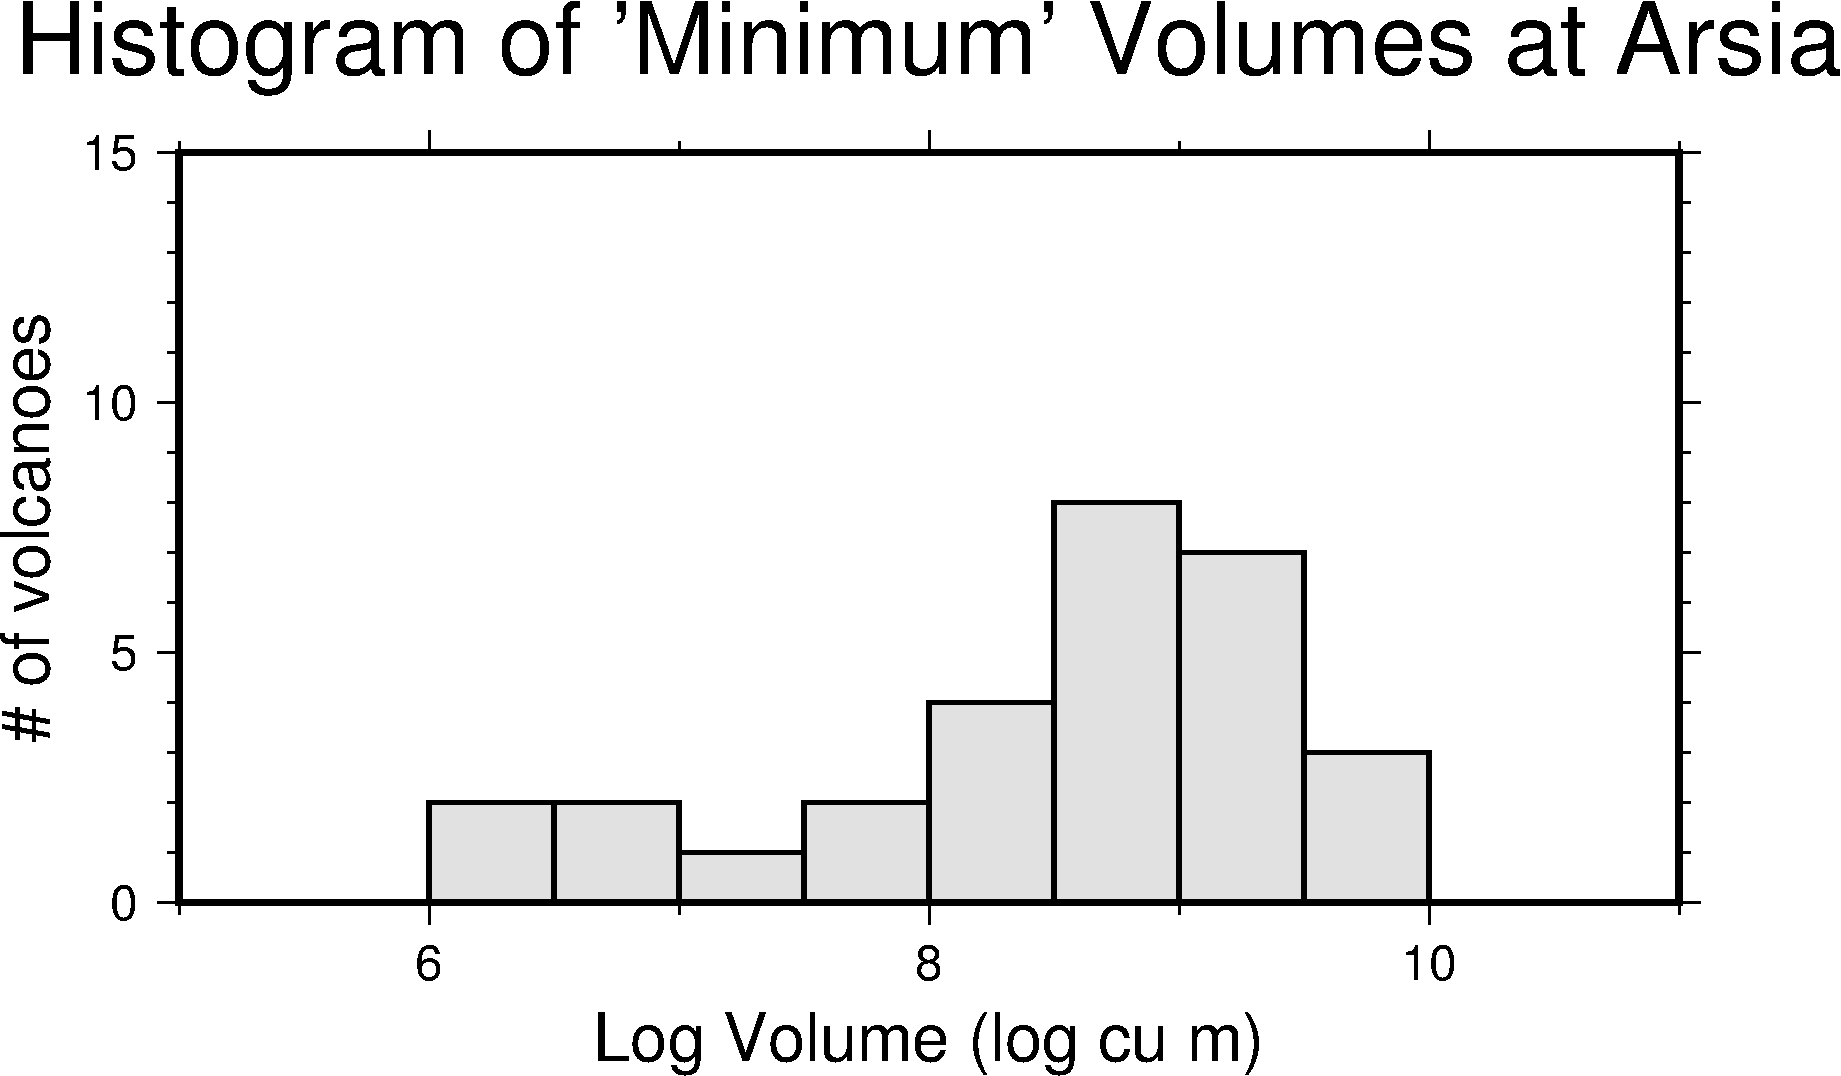
\includegraphics[width=0.5\linewidth]{figures/volumehist.png}
\caption{Minimum estimated volumes of each lava flow using an interpolated mesh as a theoretical subsurface. All lavas are estimated to be between 10$^{-3}$-1~km$^3$, with most volumes centering around 1~km$^3$.}
\label{fig_volumehistogram}
\end{figure}

\subsection{Volcanic Event Recurrence Rate Model (VERRM)}

Together, stratigraphic information and crater retention age estimates can be consolidated to improve age uncertainty estimation for volcanic events. This is especially applicable to recent volcanic landforms on Mars as crater-based dates alone might be biased due to crater burial, local topography, or secondary crater background populations \citep{robbins2011volcanic,platz2011eruption}.

To accomplish the task of constraining modeled age estimates with stratigraphy, and ultimately to describe the repose interval of volcanic events in the region, we have devised an algorithm, which we call the Volcanic Event Recurrence Rate Model (VERRM). VERRM implements a Monte Carlo algorithm that assigns a potential age to each volcanic event by defining an event age distribution function, $A$, with an event's modeled crater retention rate age and age uncertainty, as reported by Craterstats2. The age distribution function for each event is modeled as a Gaussian distribution, which is a suitable for the events in this study as they are relatively recent and the crater impact rate during the time of their emplacement is thought to be constant \citep{vaucher2009volcanic}. The initial age function is given as $A_i(\mu_i,\sigma_i^2)$ where $\mu$ is the estimated age determined by crater retention and σ is the uncertainty of the estimated age of cataloged event i. If no crater retention age estimate is given (e.g. for smaller flows with an insignificant number of impact craters), the initial age function is assumed to be a uniform probability function bounded by a minimum and maximum possible age described next.

VERRM then constrains A with a binary stratigraphy function, with possible ages having a value of 1 and ages outside an acceptable age range having a value of 0. Possible ages are defined by previously dated events in the VERRM simulation; stratigraphically higher events connected to the event at hand give a minimum age of the stratigraphy function, while lower events give a maximum age. If no stratigraphically-related events have been dated, the minimum age bound is set to the present, and the maximum age bound is set to three times older than the oldest crater retention rate modeled age in this field (330 Ma), or 1 Ga.

The normalized product of the the Gaussian age function and the binary stratigraphy function gives an age distribution function which does not violate stratigraphy but is informed by crater retention age estimates. This function is sampled to date an event and the process repeats for the next event. By repeating this process 10,000 times, the potential age ranges for each event is determined.

\paragraph{Recurrence rate calculation} Volcanic recurrence rate RR at any time $t$ is modeled for each MC solution as
\begin{equation}
\text{RR}(t) = \frac{n-1}{\text{max}\{\mathbf{T}\} - \text{min}\{\mathbf{T}\}}
\label{eq_RR}
\end{equation}
where $n$ is an even number and $\mathbf{T}$ is the set of ages of $n$ events temporally surrounding $t$. Events whose ages are elements of set $\mathbf{T}$ are identified as the closest $n/2$ events either before or after $t$. The even number $n$ is essentially a local window in time, and $n-1$ is the number of recurring events between $\text{max}\{\mathbf{T}\}-\text{min}\{\mathbf{T}\}$ after the earliest event occurrence. Note that all times $t$ laying between two temporally consecutive events will have the same set $\mathbf{T}$ and will therefore have the same calculated recurrence rate.

The set $\mathbf{T}$ is also modified for early and late times in the MC solution, where there are fewer than $n/2$ events on each side of the time period of interest. For times before the earliest event in an individual simulation (i.e. where $t$ is greater than the time of the oldest age assigned to an event), $\mathbf{T}$ includes the earliest $n-1$ events and time $t$. When $t$ falls in time between the earliest event and the $n/2^{\text{th}}$ event to occur in the simulation, $\mathbf{T}$ includes the first $n$ events. Likewise, for later (i.e. more recent) times, where $t$ is more recent than the earliest event, $\mathbf{T}$ includes both $t$ and the most recent $n-1$ events. Where $t$ falls in time between the most recent event and the $n/2^{\text{th}}$ most recent event, $\mathbf{T}$ is the set of the most recent $n$ events. For the cases where $t$ is at the same time as the earliest or latest events, $\mathbf{T}$ will be the set of times of the $n$ earliest or latest events, respectively.

While recurrence rate for any one MC simulation might be bad, the range of recurrence rates for all simulations can provide a confidence envelope of recurrence rate with respect to time. The recurrence rate for the field is defined as the median recurrence rate of all simulations over time, with a 95\% confidence envelope serving as the rate's uncertainty.

\paragraph{Volume flux calculation} Volume flux is also modeled with the VERRM output. Each event is assigned a volume (discussed above in section \ref{sec_volume}) for the lava flow it produced. Volume flux for the field is defined as the volume of erupted lava per million year time bin. A 95\% confidence envelope and median flux through time are obtained using all MC solutions.


	\begin{table}[h!]
	\centering
	\caption{Lava Flow Age Information}
	\begin{tabular}{l c c c c c}
		\toprule
			 & \multicolumn{2}{c}{Vent Location}  & Modeled & Overlying & Underlying\\
			Flow & Long. & Lat. & Age (Ma) & Flows & Flows\\
		\midrule
			v00 & -120.48$^{\circ}$ & -10.09$^{\circ}$ & 98.4$\pm$27 & --- & 02,01\\
			v01 & -120.55 & -10.02 & 71.4$\pm$41 & 00,02 & ---\\
			v02 & -120.45 & -9.98 & 117$\pm$12 & 00 & 01,03,04\\
			v03 & -120.81 & -9.76 & 99.1$\pm$15 & 02,07 & 04\\
			v04 & -120.45 & -9.78 & 126$\pm$18 & 02,03 & 05\\
			v05 & -120.30 & -9.45 & 145$\pm$17 & 04,07,10 & 06\\
			v06 & -120.33 & -9.41 & 122$\pm$49 & 05,10 & 11\\
			v07 & -120.82 & -9.65 & 94.7$\pm$11 & 09 & 03,05\\
			v08 & -120.23 & -9.30 & --- & 11,10 & ---\\
			v09 & -120.92 & -9.30 & 218$\pm$110 & --- & 07\\
			v10 & -120.24 & -9.42 & 102$\pm$9.3 & --- & 05,06,08,11,13\\
			v11 & -120.17 & -9.26 & 154$\pm$22 & 06,10,13 & 08\\
			v12 & -120.24 & -9.03 & 134$\pm$12 & 13 & 14\\
			v13 & -120.17 & -8.99 & 146$\pm$12 & 10,17 & 12,15,11\\
			v14 & -120.44 & -8.87 & 122$\pm$32 & 12,15 & ---\\
			v15 & -120.08 & -8.81 & 117$\pm$13 & 13,17 & 14,16,21\\
			v16 & -119.92 & -8.65 & 313$\pm$110 & 15,17 & 21\\
			v17 & -119.90 & -8.63 & 148$\pm$18 & --- & 13,15,16,21,25,28\\
			v18 & -120.46 & -8.55 & 186$\pm$53 & 20,21 & ---\\
			v19 & -120.36 & -8.46 & --- & 20,21 & 23\\
			v20 & -120.40 & -8.46 & 186$\pm$53 & 21 & 18,19,23\\
			v21 & -120.06 & -8.63 & 146$\pm$16 & 15,16,17 & 20,18,19,23,22,25\\
			v22 & -119.88 & -8.44 & 73.2$\pm$36 & 21,25 & ---\\
			v23 & -120.25 & -8.40 & 135$\pm$20 & 19,20,21 & 26,27\\
			v24 & -119.92 & -8.32 & --- & 25 & ---\\
			v25 & -119.79 & -8.37 & 104$\pm$16 & 17,21 & 22,24,28\\
			v26 & -120.21 & -8.21 & --- & 23 & ---\\
			v27 & -120.55 & -8.17 & 112$\pm$25 & 23 & ---\\
			v28 & -119.57 & -8.52 & 158$\pm$24 & 17,25 & ---\\
		\bottomrule
	\end{tabular}
	\label{tab_agedatabase}
	\end{table}


	\begin{table}[h!]
	\centering
	\caption{Lava Flow Morphometry}
	\begin{tabular}{l c c c c c c}
		\toprule
			 & \multicolumn{2}{c}{Vent Location}  & Area & \multicolumn{3}{c}{Volume Estimates$^*$ (km$^3$)}\\
			Flow & Long. & Lat. & (km$^2$) & subs. model & 10~m & 80~m\\
		\midrule
			v00 & -120.48$^{\circ}$ & -10.09$^{\circ}$ & 102.27 & 0.37 & 1.0 & 8.2\\
			v01 & -120.55 & -10.02 & 31.21 & 0.032 & 0.31 & 2.5\\
			v02 & -120.45 & -9.98 & 538.86 & 2.3 & 5.4 & 43\\
			v03 & -120.81 & -9.76 & 283.32 & 0.91 & 2.8 & 23\\
			v04 & -120.45 & -9.78 & 242.29 & 1.6 & 2.4 & 19\\
			v05 & -120.30 & -9.45 & 353.98 & 0.89 & 3.5 & 28\\
			v06 & -120.33 & -9.41 & 69.40 & 0.31 & 0.69 & 5.6\\
			v07 & -120.82 & -9.65 & 479.32 & 5.0 & 4.8 & 38\\
			v08 & -120.23 & -9.30 & 4.00 & 0.0017 & 0.04 & 0.32\\
			v09 & -120.92 & -9.30 & 21.08 & 0.013 & 0.21 & 1.7\\
			v10 & -120.24 & -9.42 & 858.69 & 3.2 & 8.6 & 69\\
			v11 & -120.17 & -9.26 & 228.09 & 1.0 & 2.3 & 18\\
			v12 & -120.24 & -9.03 & 528.14 & 1.6 & 5.3 & 42\\
			v13 & -120.17 & -8.99 & 679.49 & 3.2 & 6.8 & 54\\
			v14 & -120.44 & -8.87 & 96.78 & 0.14 & 0.97 & 7.7\\
			v15 & -120.08 & -8.81 & 460.75 & 2.5 & 4.6 & 37\\
			v16 & -119.92 & -8.65 & 18.11 & 0.0053 & 0.18 & 1.4\\
			v17 & -119.90 & -8.63 & 300.03 & 0.64 & 3.0 & 24\\
			v18 & -120.46 & -8.55 & 64.29 & 0.16 & 0.64 & 5.1\\
			v19 & -120.36 & -8.46 & 13.12 & 0.0047 & 0.13 & 1.0\\
			v20 & -120.40 & -8.46 & 70.51 & 0.14 & 0.71 & 5.6\\
			v21 & -120.06 & -8.63 & 354.97 & 1.6 & 3.5 & 28\\
			v22 & -119.88 & -8.44 & 53.20 & 0.31 & 0.53 & 4.3\\
			v23 & -120.25 & -8.40 & 204.71 & 0.53 & 2.0 & 16\\
			v24 & -119.92 & -8.32 & 11.70 & 0.037 & 0.12 & 0.94\\
			v25 & -119.79 & -8.37 & 281.19 & 2.0 & 2.8 & 22\\
			v26 & -120.21 & -8.21 & 5.61 & 0.0026 & 0.056 & 0.45\\
			v27 & -120.55 & -8.17 & 158.16 & 1.8 & 1.6 & 13\\
			v28 & -119.57 & -8.52 & 176.53 & 0.58 & 1.8 & 14\\
		\bottomrule
		\multicolumn{6}{p{0.65\linewidth}}{$^*$The three volume estimates are found using 1) a modeled subsurface, 2) assuming an average thickness of 10~m and 3) 80~m.}
	\end{tabular}
	\label{tab_morphdatabase}
	\end{table}

\section{Results}

	\begin{figure}[h!]
		\centering
		\begin{gnuplot}[terminal=latex, terminaloptions=rotate]
			unset key
			set size 1,1
			set xlabel "Time before present, Ma" rotate by 90
			set ylabel "Recurrence rate (events Myr$^{-1}$)"
			set xrange [350:0]
			set y2tics 0.25
			set ytics 0.25
			set xtics 100
			plot "Arsia_Mons_FOR_PUBLICATION_MA_RR_4_crater_neighbor.dat" using 1:2 with lines lt 4, "Arsia_Mons_FOR_PUBLICATION_MA_RR_4_crater_neighbor.dat" using 1:4 with lines lt 4, "Arsia_Mons_FOR_PUBLICATION_MA_RR_4_crater_neighbor.dat" using 1:3 with lines lt 5
		\end{gnuplot}
		\caption{Modeled recurrence rate of effusive volcanic events in Arsia Mons Caldera for the last 350~Ma. The median recurrence rate of MC simulations is plotted in bold; a 95\% confidence envelope is plotted as dots. For the 29 observed flows, recurrence rate of activity reached a peak at 150~Ma, producing an average of 1 new edifice per 4 Myr (one every 1-9 Myr within 95\% confidence). Activity then waned until 10-90~Ma, when volcanism ceased.}
		\label{fig_VERRMRR}
	\end{figure}
	
The 29 lava flows in our catalog are mapped to cover 6700 km$^2$, $\sim$70\%, of the caldera, representing the majority of surface lavas within the caldera walls (Figure \ref{fig_lavamap}). Each flow has at least one neighboring flow, which enables a stratigraphic web to be produced that connects all volcanic events to other events \ref{fig_stratweb}. Age estimates modeled from crater retention ranged from 71-313~Ma, though the youngest and oldest ages are not observed at the top or bottom of the stratigraphic web. This indicates that the crater ages might not be well constrained for small and relatively young surface units on Mars, but that ages for these units might be better constrained with stratigraphic information. These data are detailed for each edifice in Table \ref{tab_agedatabase}.
	
	\begin{figure}[ht]
		\centering
		\begin{gnuplot}[terminal=latex, terminaloptions=rotate]
			unset key
			set size 1,1
			set xlabel "Time before present, Ma" rotate by 90
			set ylabel "Volume Flux (km$^3$ Myr$^{-1}$)"
			set xrange [350:0]
			set y2tics 0.5
			set ytics 0.5
			set xtics 100
			plot "Arsia_Mons_MIN_VOLUME_CORRECTED_time_predict_crater_neighbor.dat" using 1:2 with lines lt 4, "Arsia_Mons_MIN_VOLUME_CORRECTED_time_predict_crater_neighbor.dat" using 1:4 with lines lt 4, "Arsia_Mons_MIN_VOLUME_CORRECTED_time_predict_crater_neighbor.dat" using 1:3 with lines lt 5
		\end{gnuplot}
		\caption{Modeled volume flux for the latest effusive activity within Arsia Mons Caldera, using a subsurface model under each lava flow to calculate edifice volume. The median flux of the MC simulations is plotted in bold; a 95\% confidence envelope is plotted as dots. By 150~Ma, 0.1 km$^3$ of magma is modeled to have been delivered to the surface every million years, and the delivery rate might have doubled (0.2 km$^3$~Myr$^{-1}$) by 100 Ma before quickly waning to quiescence around 90~Ma.}
		\label{fig_VERRMMINVOL}
	\end{figure}
	\begin{figure}[h!]
		\centering
		\begin{gnuplot}[terminal=latex, terminaloptions=rotate]
			unset key
			set size 1,1
			set format xy "$%g$"
			set xlabel "Time before present, Ma" rotate by 90
			set ylabel "Volume Flux, 10 m flows (km$^3$ Myr$^{-1}$)"
			set y2label "Volume Flux, 80 m flows (km$^3$ Myr$^{-1}$)"
			set xrange [350:0]
			set yrange [0:4.5]
			set y2range [0:36]
			set ytics 1
			set y2tics 8
			set xtics 100
			plot "Arsia_Mons_10m_THICK_CORRECTED_time_predict_crater_neighbor.dat" using 1:2 with lines lt 4, "Arsia_Mons_10m_THICK_CORRECTED_time_predict_crater_neighbor.dat" using 1:4 with lines lt 4, "Arsia_Mons_10m_THICK_CORRECTED_time_predict_crater_neighbor.dat" using 1:3 with lines lt 5
		\end{gnuplot}
		\caption{Modeled volume flux for the latest effusive activity within Arsia Mons Caldera, assuming mapped units have an average thickness of 10~m (left axis) or 80~m (right axis). The median flux of the MC simulations is plotted in bold; a 95\% confidence envelope is plotted as dots. Contrasted with the subsurface-model estimated volume results in Figure \ref{fig_VERRMMINVOL}, volume flux is modeled here to remain relatively constant between 150-100~Ma. The median flux for these 50 million years is estimated to be 0.4~km$^3$~Myr$^{-1}$ assuming 10~m thick units or 3 ~km$^3$~Myr$^{-1}$ for 80~m thick units.}
		\label{fig_VERRMAREA}
	\end{figure}
	
Lava flow volume estimates using the subsurface modeling method range from $1.6\cdot 10^{-3}$ to 5 km$^3$, with an average of 1.1 km$^3$ per flow (Figure \ref{fig_volumehistogram}). The total volume using this method, again assumed to be a minimum volume estimate, is 31 km$^3$. Average flow thickness for the 29 flows is 4.6~m, which is thinner than the thinnest flows identified by \citet{mouginis2008lava} by a factor of two. Individual volumes are reported in Table \ref{tab_morphdatabase}. We also report the volumes of each flow assuming an average thickness of 10 and 80~m, which might be more reasonable volume bounds. Assuming these two thicknesses gives the flow field a total modeled volume of 67 or 540~km$^3$, respectively.

%%%ALL YOU HAVE TO DO IS WRITE A FEW LINES ABOUT VERRMMMM COULD IT BE SO HARD? THEN MODIFY THE DISCUSSION AND CONCLUSION AND SEND IT OFF. THEN WORK ON LAVA
Modeling the recurrence rate of volcanism using both crater retention age dating and the stratigraphic relationships between neighboring lava flows (Figure \ref{fig_stratweb}) in the VERRM algorithm constrains the intra-caldera activity to the most recent 200~Ma. The 29 mapped volcanic events are modeled to have begun erupting around 200~ma, eruption frequency waxed to 150~Ma, and monotonically waned to 10-90~Ma (Figure \ref{fig_VERRMRR}). The peak recurrence rate, estimated as the median of 10,000 MC solutions, was 0.25 events per million years, or an average of 1 vent being created each 4 ~Myr. The 95\% confidence envelope of the recurrence rate through time is generally a factor of 2-4. This means that at peak activity, our model estimates a recurrence rate of vent formation of 0.1-1 events per Myr. Volcanism then likely ceased after 90~Ma, but might have ended as recently as 10~Ma, with a median end age of 60~Ma. These 29 volcanic edifices would have then been emplaced over a time period of 110-190~Myr.

The long term magma supply rate to the surface, or volume flux, is modeled using three separate estimated volumes for each edifice, listed in Table \ref{tab_morphdatabase}. First, volume estimates calculated by modeling a subsurface under each edifice and subtracting the subsurface from the overlying topography is used as edifice volumes in modeling volume flux. This model of volume flux through time is shown in Figure \ref{fig_VERRMMINVOL}. The median flux of all MC solutions here is modeled to increase to a delivery rate of 0.1 km$^3$~Myr$^{-1}$ at 150~Ma before doubling to 0.2 km$^3$~Myr$^{-1}$ around 100~Ma. The delivery rate then dies off quickly. There is significant uncertainty in this model, so that the peak discharge could have occurred at 150~Ma as well. The confidence envelope of 95\% of MC solutions for this model is roughly an order of magnitude on either side.

The other two edifice volume models assume that edifices have an average thickness of either 10 or 80~m. These models of volume flux are illustrated in Figure \ref{fig_VERRMAREA}, where the left y-axis is scaled to 10~m thick units and the right y-axis is scaled to represent 80~m thick units. This result suggests, like the flux model using subsurface-estimated volumes, that the  magma delivery rate grew to 150, but unlike the other flux model, the delivery rate remained relatively steady until 90-100~Ma, when it declined. If units are assumed to be 10~m thick, this delivery rate plateau is 0.4 km$^3$~Myr$^{-1}$. If units are 80~m thick, the rate would be 3~km$^3$~Myr$^{-1}$.

%mention that Figure 6 shows that the biggest volumes were young but not youngest! lavas.
%Talk about how the peak isn't present for the other models.

\section{Discussion}
The main finding in this study is that emplacement of the observable volcanic edifices in Arsia Mons caldera likely occurred between 200 and 10-90~Ma, and reached a maximum rate of vent creation at 150~Ma. A major complication to the modeled onset of activity (200~Ma) is the significant likelihood that previous volcanic vents are simply buried by the low shield lavas of the mapped 29 volcanoes. Several scenarios are possible for times before 150~Ma. One possibility is that these 29 volcanoes began a new, unique period of activity, resurfacing an old caldera after a large hiatus in Arsia volcanism. This would be in-line with the recurrence rate as modeled by the VERRM algorithm, since the algorithm only uses the 29 cataloged volcanic vents. Another possibility is that the mapped units overlay an uncountable number of similar low shields, which were emplaced at the same rate as the mapped shields were. Yet another scenario would be that these vents occured immediately after a distinct style of volcanism, perhaps evidence of large edifice-building eruptions. These two scenarios would invalidate the modeled rise in volcanic recurrence rate between 200-150~Ma. Because it is not currently possible to detect what lay beneath the mapped low shields, it is unknown whether the rise in recurrence rate is real or not. However, after 150~Ma the most recent volcanism can be better constrained as fewer recent vents should be buried. Because of this, the 100~Myr period of waning volcanic recurrence shown in Figure \ref{fig_VERRMRR} is more likely to be correctly modeled.

The differences between volume flux models in Figures \ref{fig_VERRMMINVOL} and \ref{fig_VERRMAREA} might illustrate bias in estimating edifice volume. By calculating volume based on a constant thickness and mapped area (Figure \ref{fig_VERRMAREA}), volume flux remains steady from 150-100~Ma, while recurrence rate decreases. This would indicate that older eruptions were less voluminous than recent eruptions, though it might also be a factor of older low shields having a smaller exposed area simply because they are embayed by younger flows. This bias might be exacerbated by modeling the edifice subsurface using gridded topographic data, which was the method used in modeling volume flux in Figure \ref{fig_VERRMMINVOL}. Small areas are more likely to be interpolated less accurately in the MOLA topographic dataset, and the topographic rise might therefore be less pronounced, leading to systematically less volumes for small areas. It is important to note, however, that in both volume flux models, magma discharge decreases quickly after 100~Ma, while event recurrence rate continues to decline steadily for 10-90~Myr. This is because, though the largest edifices are high stratigraphically, the uppermost stratigraphic edifices are relatively small. This pattern might be evidence that as recurrence rate of vent creation waned, the size of eruptions also waned at the tail end of volcanic activity in the Arsia Mons caldera.

\subsection{Comparisons to other studies}

Modeled ages of these flows with our crater counts lay between 70-400 Ma, with uncertainties reported by craterstats2 to be between 10-100 Myr. Our ages confirm modeled ages produced by other authors, where we find the crater-derived model age of the entire caldera to be 123 Ma, similar to \citet{neukum2004recent}, \citet{werner2009global} and \citep{robbins2011volcanic}. \citet{robbins2011volcanic} also used crater retention rates (for D≥93 m) to date a single endogenous crater located within the caldera at 9.70°S, 239.18°E as having an age of 97$\pm$49 Ma. We independently date the lava flow associated with this vent to have an age of 99$\pm$15 Ma (Figure \ref{fig_craterct}).

\begin{figure}
\centering
\begin{subfigure}{.33\textwidth}
  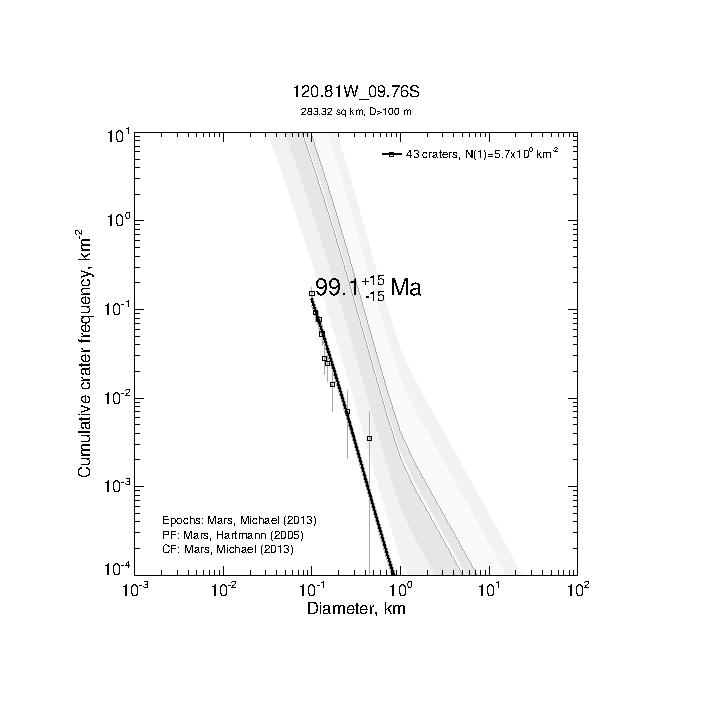
\includegraphics[width=\linewidth,clip,trim=1cm 1cm 1.5cm 1cm]{figures/craterstats/120-81W_09-76S_100m_cum.eps}
\end{subfigure}%
\begin{subfigure}{.33\textwidth}
  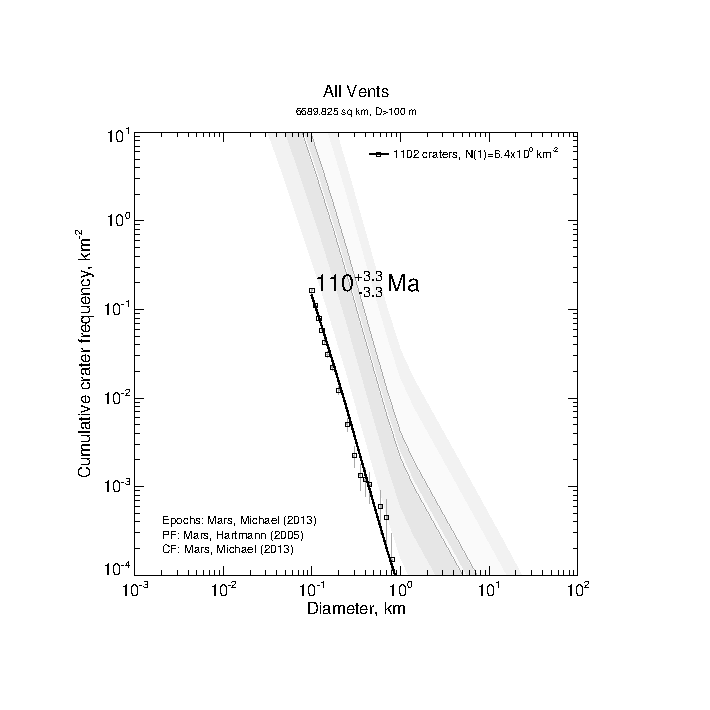
\includegraphics[width=\linewidth,clip,trim=1cm 1cm 1.5cm 1cm]{figures/craterstats/arsia_all29_cum.eps}
\end{subfigure}
\begin{subfigure}{.33\textwidth}
  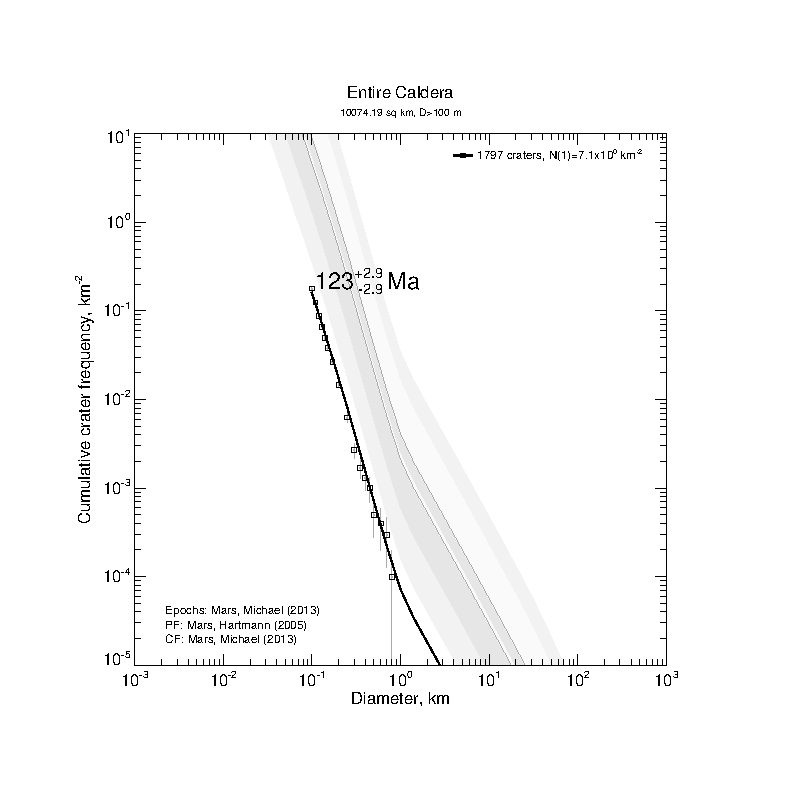
\includegraphics[width=\linewidth,clip,trim=1cm 1cm 1.5cm 1cm]{figures/craterstats/arsia_fullarea_100m_cum.eps}
\end{subfigure}
\caption{Cumulative crater frequency distributions for (left) one lava flow, (center) all mapped lava flows, (right) the entire caldera). The example flow, v03 in our database, had been previously estimated to be 97$\pm$49 Ma from crater counting performed on a HiRISE image \citep{robbins2011volcanic}. Our age of 99$\pm$15 Ma agrees with this previous finding. The age of the entire caldera also generally agrees with previous estimates of 130~Ma. The mapped vents plot younger than the entire caldera, which is expected as they are the most recent resurfacing events on the caldera.}
\label{fig_craterct}
\end{figure}

Our initial VERRM results suggest that the Arsia field might have been active for 110-190 Myr, ending between 10-90 Mya (Figure \ref{fig_VERRMRR}). If 67 or 540 km$^3$ of basalt (given average lava thickness of 10 or 80~m) was emplaced as lavas during this time, the long-term magma discharge rate of the field would have maintained 0.4 or 3 km$^3$ Myr$^{-1}$ (400-3000~m$^3$~yr$^{-1}$ or $10^{-5}$-$10^{-4}$~m$^3$~s$^{-1}$) for most of the activity (Figure \ref{fig_VERRMAREA}). This is two to three orders of magnitude less active than the magma flux estimated for Central Elysium Planitia, calculated by \citet{vaucher2009volcanic} to be $1.4\cdot 10^{-2}$ to $1.8\cdot 10^{-2}$~m$^3$~s$^{-1}$ over the most recent 234 Myr, through similar volume estimates of lava flows and a crater retention rate study. Our estimate is also 5 orders of magnitude lower than the average magma flux (30 m$^3$ s$^{-1}$) \citet{wilson2001evidence} calculated would be needed to charge the most recent magma chamber under Arsia Mons. If we employ the same 8.5:1 intrusive/extrusive ratio used by \citet{greeley1991magma}, the total magma production at depth during the emplacement of the caldera flows would be $10^{-4}$-$10^{-3}$~m$^3$~s$^{-1}$. This is still much lower than the estimated flux necessary to sustain a magma chamber, and is two or three orders of magnitude smaller than the average flux needed to build Arsia Mons in 1 Gyr, 0.05 m$^3$ s$^{-1}$ \citep{wilson2001evidence}.

Time-averaged recurrence can be estimated by dividing the total elapsed time of volcanic activity by number of events. For instance, \citet{richardson2013volcanic} identified 263 monogenetic volcanic vents within Syria Planum, which were interpreted to be emplaced from 3.6-2.9 Ga, or 700 Myr. If volcanism were constant in that area, a new volcanic vent would have been formed every 2.7 Myr. In a graben on the northwest flank of Arsia, \citet{mouginis2008lava} mapped $>$1000 lava flows and estimated construction rates of 290 and 435 million years, based on the time to build all of Arsia Mons. This would correspond to a recurrence of at least one episode of lava emplacement every 290 or 440 kyr. A time-averaged recurrence for our 29 vents, created over 110-190 Myr, would be one event every 4-7 Myr. This alone would imply that the latest volcanic activity on Arsia Mons was much closer in style to the volcanism on Syria Planum than during the main constructional phases of Arsia Mons.

\subsection{Effects on tropical mountain glaciers on Arsia Mons}

In the past decade, studies have interpreted fan-shaped deposits on the western flanks of the Tharsis Montes to be recent glacial deposits, due to the presence of fresh moraines and possible stranded ice blocks, analogous to kettles on Earth \citep{shean2007recent,kadish2014middle,scanlon2015remnant}. The material on these broad deposits have been dated by \citet{kadish2014middle} to have been emplaced around 200 Ma. \citet{scanlon2015volcanism} identified fan-shaped deposits on the western flank of Arsia Mons which contain evidence of basal melting in clear association with sub-glacial volcanic eruptions. 

Recent analysis of smooth facies deposits to the northwest of the Arsia summit has provided evidence that tropical mountain glaciers are, in fact, extant and covered in ash \citep{scanlon2015remnant}. The penetration depth of viscously relaxed ring-mold craters on these deposits indicates a maximum material blanket thickness of less than 230 m over tens to hundreds of meters of ice or ice-rich material \citep{head2014preservation}. A large portion of this insulating material might in fact be volcanic ash \citep{wilson1994mars,mouginis2002prodigious}.

The presence of volcanic ash on remaining tropical mountain glaciers on the flank of Arsia might be a result of the most recent volcanism in the Arsia caldera. If this is the case, our volume estimates would likely be severely underestimated, as a large portion of erupted material would have been transported away from the vent as tephra. However, as \citet{kadish2014middle} estimated the resurfacing age of the fan-shaped deposits to be about 200 Ma, roughly our interpreted age of onset of effusive activity within the caldera, it is possible that the ash on the flanks and the lavas in the caldera represent a transition from explosive to effusive volcanism at Arsia Mons. The provenance of the ash might be buried by the recent lavas or might be the ``parasitic calderas'' observed by \citet{crumpler1996calderas}, which form a rift of the south and north caldera walls of Arsia, in line with the shield volcanoes in our catalog.

\subsection{Transition of volcanic style and waning of Arsia volcanism}
From our findings and evidence of significant amounts of ash to the west \citep{mouginis2002prodigious}, we interpret the intra-caldera lava flows to represent the waning of activity at Arsia Mons, which effectively ended $\sim$10-90~million years ago. Preceding the formation of the large basaltic caldera, magmatic activity would have mainly been related to a large magma chamber, which was active at a heightened rate \citep{wilson2001evidence}. Dikes ascending below this chamber are expected to propagate towards the chamber and ultimately assimilate with it \citep{karlstrom2009organization}, effectively suppressing monogenetic volcanism directly above the chamber during its molten history. Instead, large events related to the central chamber would have occurred, perhaps supplying the provenance of ash now mantling ice-rich material on Arsia's west flanks.

The relatively small volumes and distributed nature of the lavas within the caldera, as well as the caldera itself, are evidence that the magma chamber has cooled and that dikes are able to ascend individually through the center of the caldera. The magma supply rate to the base of Arsia must therefore have waned to below $\sim$12~m$^3$~s$-1$ (plus or minus a factor of three) \citep{wilson2001evidence}. The long-term average surface flux of distributed volcanism in this study, $10^{-4}$-$10^{-3}$~m$^3$~s$^{-1}$, is four to five orders of magnitude below this minimum supply rate. Since at least 200~Ma individual dikes ascended to the surface, with on average 0.1-1 intersecting the caldera surface per million years at 150~Ma, creating a new vent and effusive lavas. This recurrence rate of dike ascent then slowed until 10-90~Ma, when the latest volcanic vent was formed.

\section{Conclusions}

We have modeled the recurrence rate of vent production in the Arsia Mons caldera by combining two sources of age information: crater retention and stratigraphy. By constraining crater retention age estimates for lavas emminating from each vent with stratigraphic relationships observed at flow boundaries, potential timelines of volcanic activity can be constructed. The VERRM algorithm employs a Monte Carlo method to identify the variance of potential eruption timelines, and ultimately model both recurrence rate and long-term volume flux of lavas in the caldera.

Results from the VERRM algorithm suggest that the 29 lava flows mapped in the caldera created a volcanic field that was active since at least 200~Ma and became inactive at between 10-90~Ma. The cumulative volume of flows is modeled to be 30-540~km$^3$. The magma surface delivery rate, or volume flux, of the mapped vents increased to a plateau of 0.1-3~km$^3$~Myr$^{-1}$ by 150~Ma, depending on the assumed thickness of each edifice, and might have peaked at 100~Ma before rapidly waning.

The confidence envelope for volcanic recurrence rate (Figure \ref{fig_VERRMRR}) for times older than the peak of volcanism in this study (150~Ma) is likely unreliable---while the envelope suggests that recurrence among the 29 volcanoes waxes during this time, it is beyond likely that below the 29 lava flows, other flows and volcanic vents are buried. The increasing trend in recurrence rate might be erroneous because of a lack of data on these possible buried events. However, it is likely that the waning trend observed since 150~Ma is real. This waning trend, as well as the presence of distributed lava flows in the caldera, might represent the tail-end of an episode of activity in Arsia Mons that formed the large basaltic caldera and a corresponding magma chamber hypothesized by \citet{wilson2001evidence}. 







%\begin{figure}
%\centering
%\includegraphics[width=\linewidth]{map_diff}
%\label{fig:map_diff}
%\end{figure}



\addcontentsline{toc}{section}{References}
\bibliographystyle{plainnat}
\bibliography{arsia}

\section{Appendix: cumulative crater charts}\label{sec_cccharts}
\begin{figure}[h]
\centering
\begin{subfigure}{.33\textwidth}
  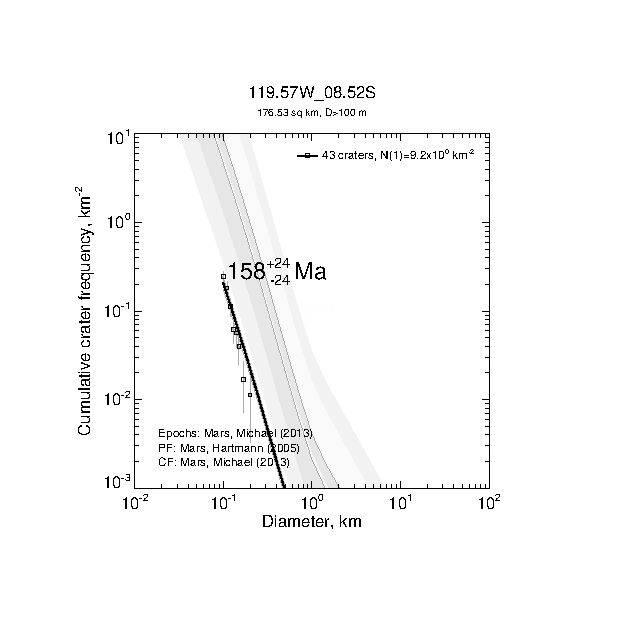
\includegraphics[width=\linewidth,clip,trim=1cm 1cm 1.5cm 1cm]{figures/craterstats/119-57W_08-52S_100m_cum.eps}
\end{subfigure}%
\begin{subfigure}{.33\textwidth}
  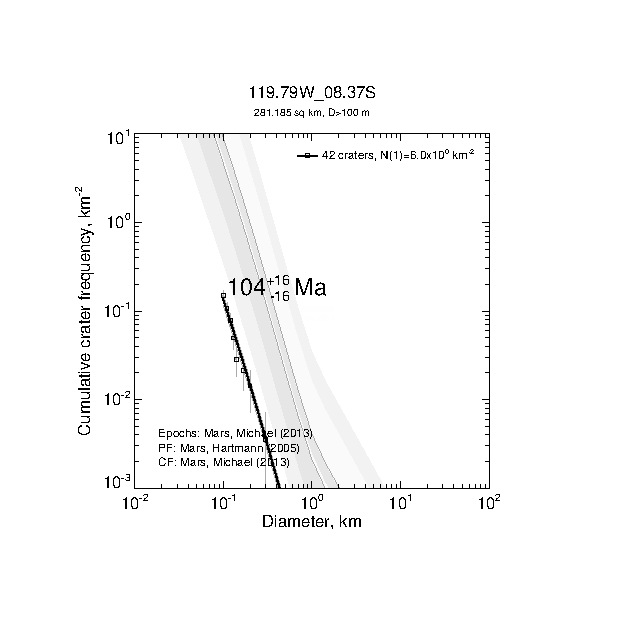
\includegraphics[width=\linewidth,clip,trim=1cm 1cm 1.5cm 1cm]{figures/craterstats/119-79W_08-37S_100m_cum.eps}
\end{subfigure}
\begin{subfigure}{.33\textwidth}
  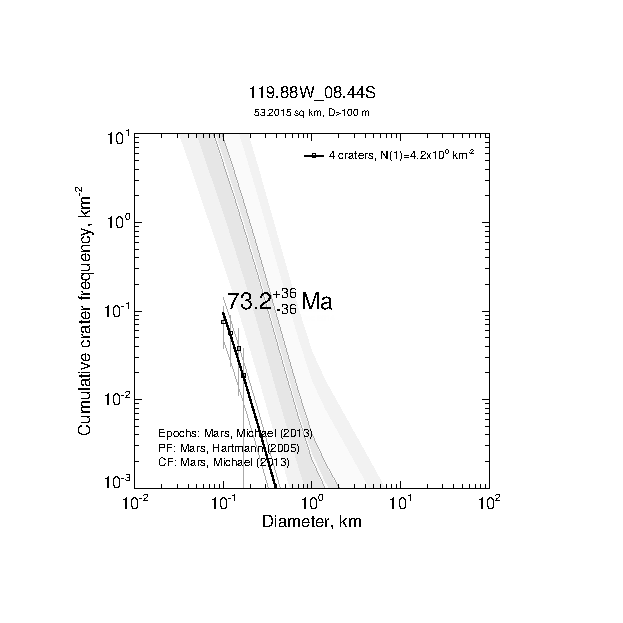
\includegraphics[width=\linewidth,clip,trim=1cm 1cm 1.5cm 1cm]{figures/craterstats/119-88W_08-44S_100m_cum.eps}
\end{subfigure}
\begin{subfigure}{.33\textwidth}
  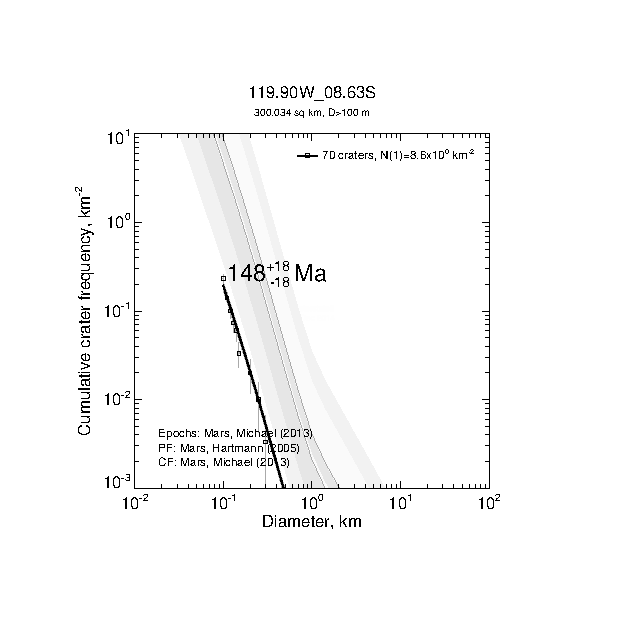
\includegraphics[width=\linewidth,clip,trim=1cm 1cm 1.5cm 1cm]{figures/craterstats/119-90W_08-63S_100m_cum.eps}
\end{subfigure}%
\begin{subfigure}{.33\textwidth}
  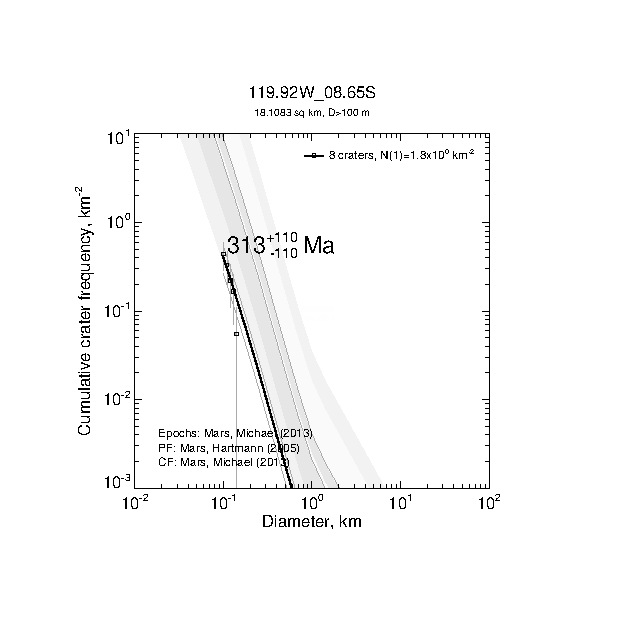
\includegraphics[width=\linewidth,clip,trim=1cm 1cm 1.5cm 1cm]{figures/craterstats/119-92W_08-65S_100m_cum.eps}
\end{subfigure}
\begin{subfigure}{.33\textwidth}
  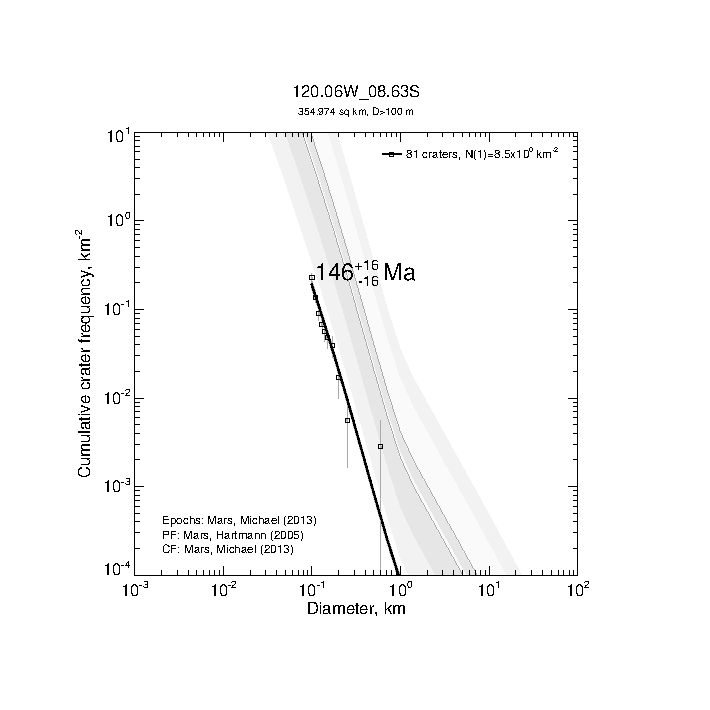
\includegraphics[width=\linewidth,clip,trim=1cm 1cm 1.5cm 1cm]{figures/craterstats/120-06W_08-63S_100m_cum.eps}
\end{subfigure}
\begin{subfigure}{.33\textwidth}
  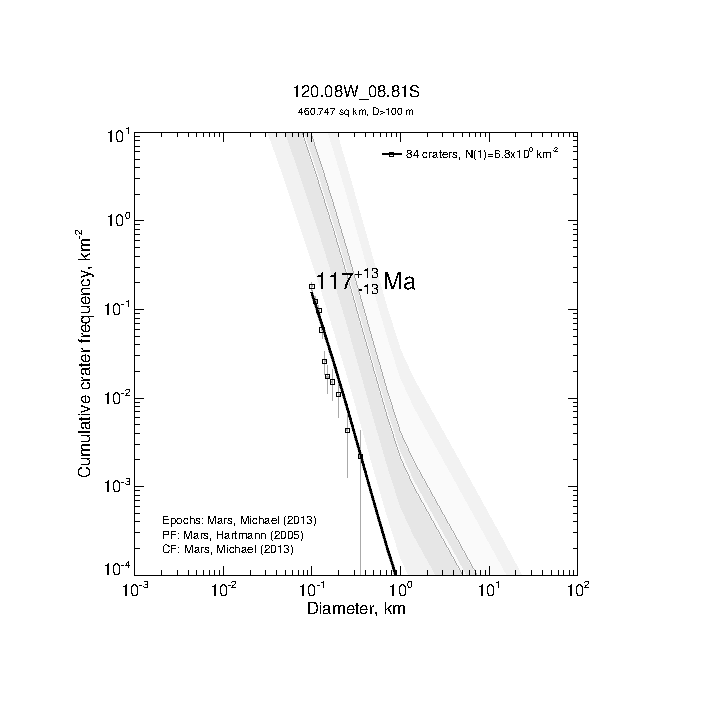
\includegraphics[width=\linewidth,clip,trim=1cm 1cm 1.5cm 1cm]{figures/craterstats/120-08W_08-81S_100m_cum.eps}
\end{subfigure}%
\begin{subfigure}{.33\textwidth}
  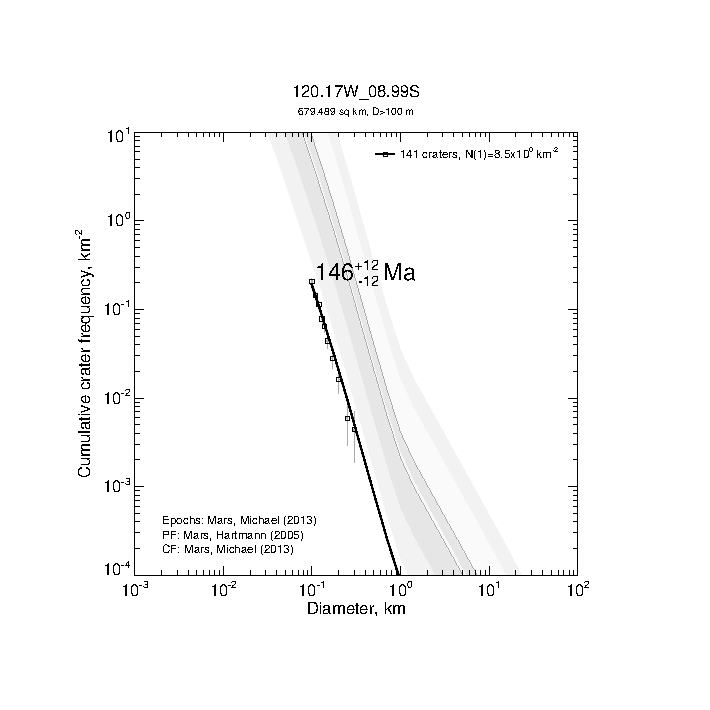
\includegraphics[width=\linewidth,clip,trim=1cm 1cm 1.5cm 1cm]{figures/craterstats/120-17W_08-99S_100m_cum.eps}
\end{subfigure}
\begin{subfigure}{.33\textwidth}
  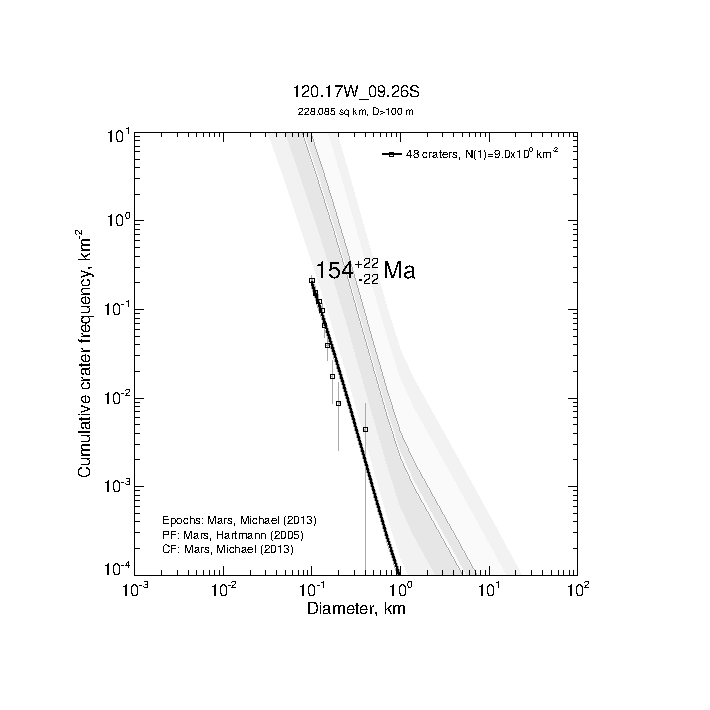
\includegraphics[width=\linewidth,clip,trim=1cm 1cm 1.5cm 1cm]{figures/craterstats/120-17W_09-26S_100m_cum.eps}
\end{subfigure}
\end{figure}

\begin{figure}[h]
\centering
\begin{subfigure}{.33\textwidth}
  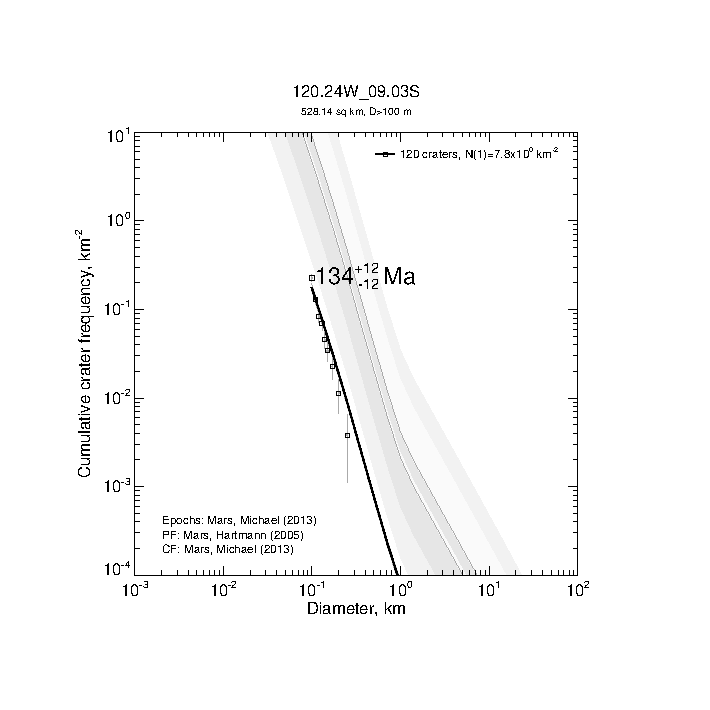
\includegraphics[width=\linewidth,clip,trim=1cm 1cm 1.5cm 1cm]{figures/craterstats/120-24W_09-03S_100m_cum.eps}
\end{subfigure}%
\begin{subfigure}{.33\textwidth}
  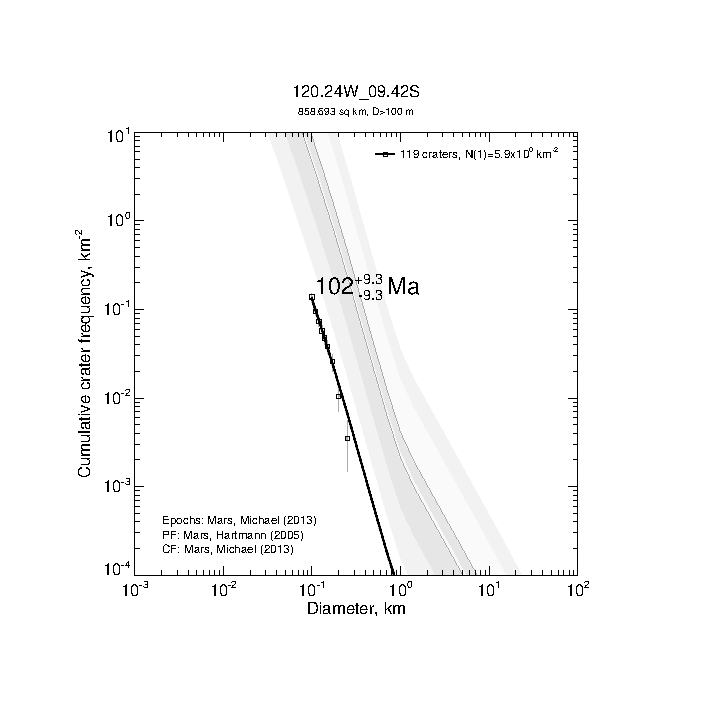
\includegraphics[width=\linewidth,clip,trim=1cm 1cm 1.5cm 1cm]{figures/craterstats/120-24W_09-42S_100m_cum.eps}
\end{subfigure}
\begin{subfigure}{.33\textwidth}
  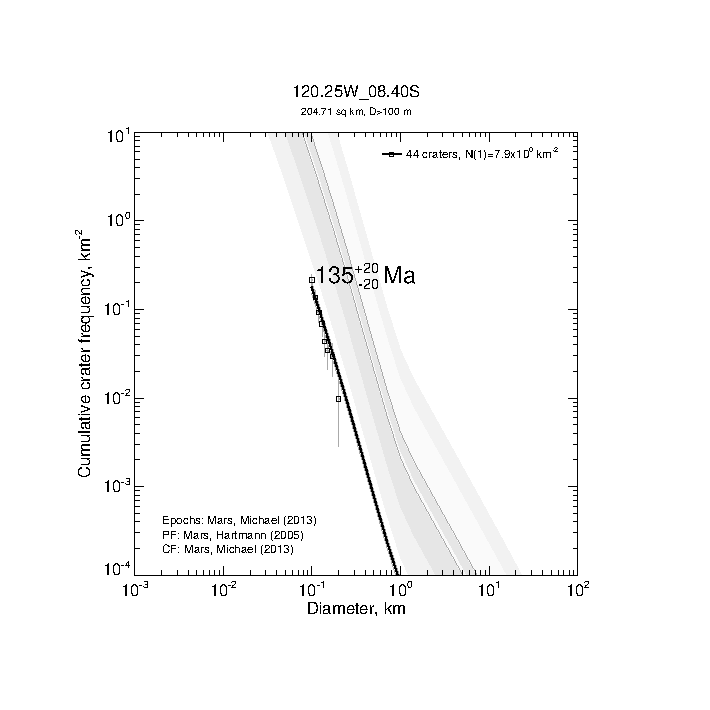
\includegraphics[width=\linewidth,clip,trim=1cm 1cm 1.5cm 1cm]{figures/craterstats/120-25W_08-40S_100m_cum.eps}
\end{subfigure}
\begin{subfigure}{.33\textwidth}
  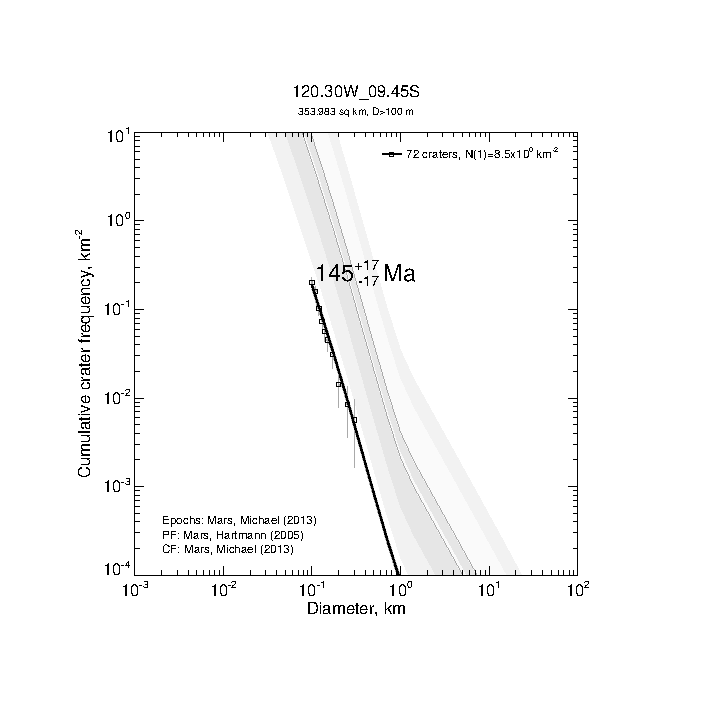
\includegraphics[width=\linewidth,clip,trim=1cm 1cm 1.5cm 1cm]{figures/craterstats/120-30W_09-45S_100m_cum.eps}
\end{subfigure}%
\begin{subfigure}{.33\textwidth}
  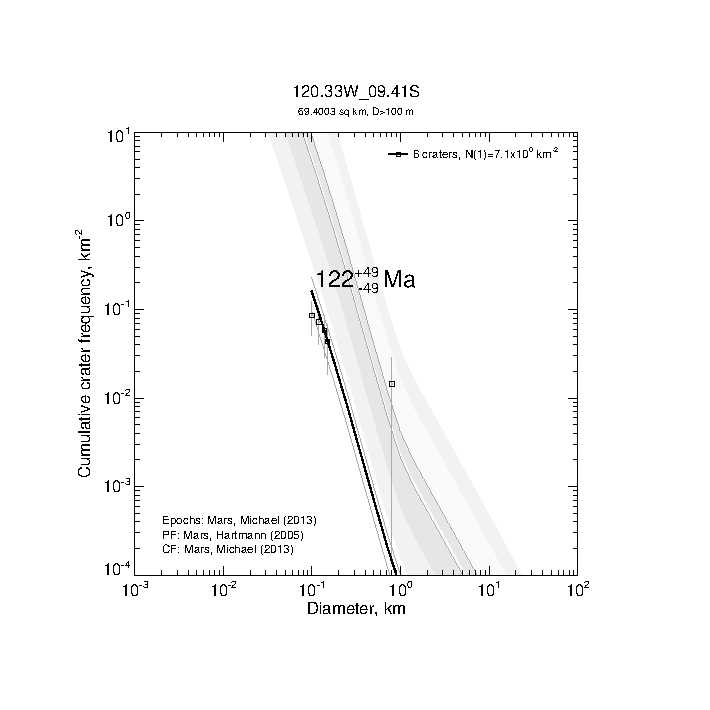
\includegraphics[width=\linewidth,clip,trim=1cm 1cm 1.5cm 1cm]{figures/craterstats/120-33W_09-41S_100m_cum.eps}
\end{subfigure}
\begin{subfigure}{.33\textwidth}
  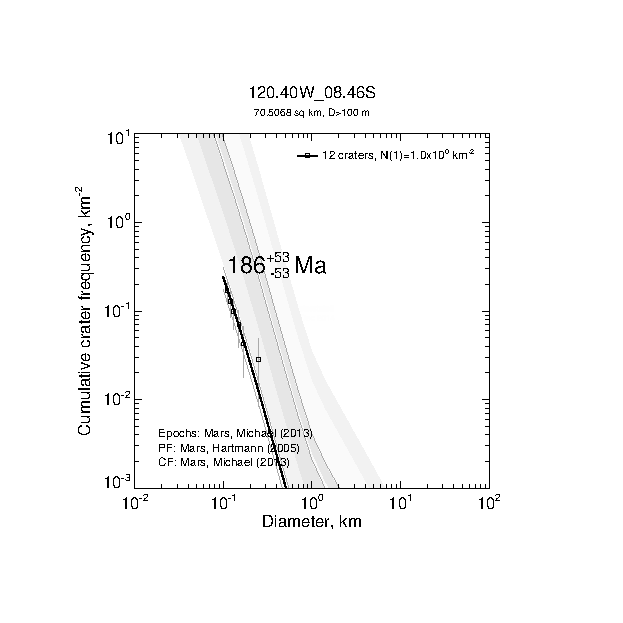
\includegraphics[width=\linewidth,clip,trim=1cm 1cm 1.5cm 1cm]{figures/craterstats/120-40W_08-46S_100m_cum.eps}
\end{subfigure}
\begin{subfigure}{.33\textwidth}
  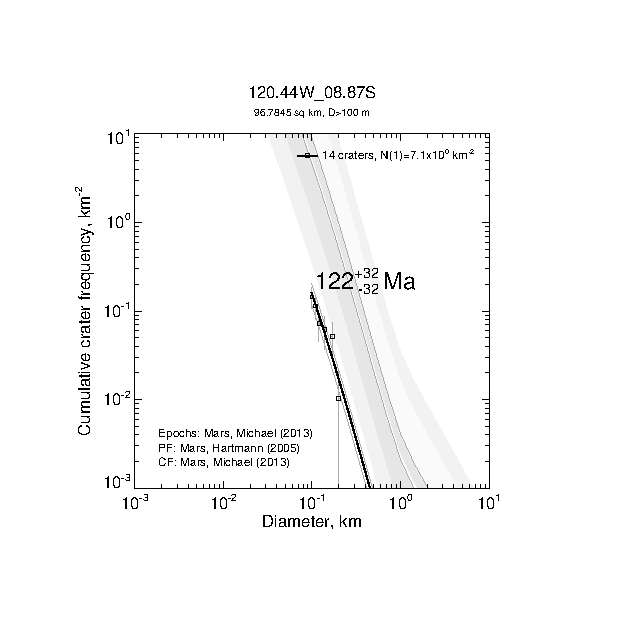
\includegraphics[width=\linewidth,clip,trim=1cm 1cm 1.5cm 1cm]{figures/craterstats/120-44W_08-87S_100m_cum.eps}
\end{subfigure}%
\begin{subfigure}{.33\textwidth}
  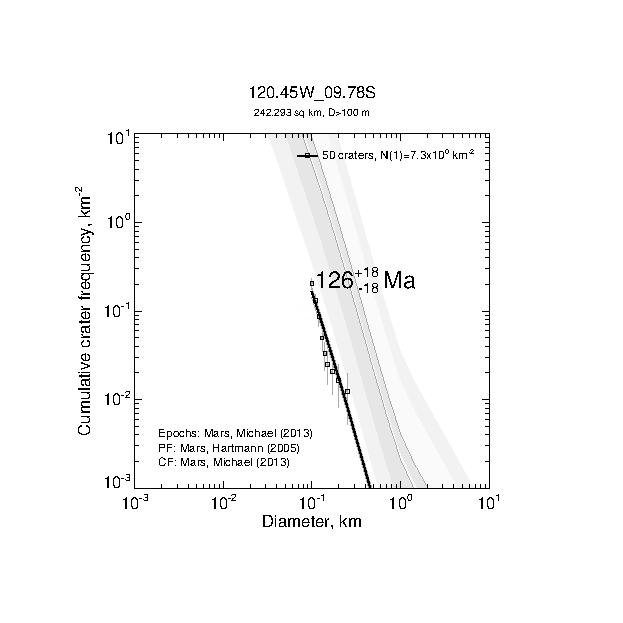
\includegraphics[width=\linewidth,clip,trim=1cm 1cm 1.5cm 1cm]{figures/craterstats/120-45W_09-78S_100m_cum.eps}
\end{subfigure}
\begin{subfigure}{.33\textwidth}
  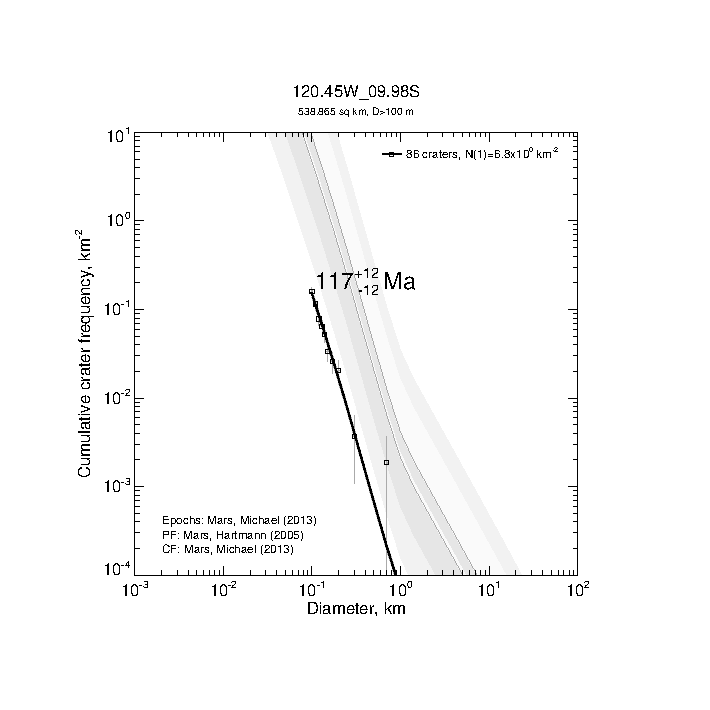
\includegraphics[width=\linewidth,clip,trim=1cm 1cm 1.5cm 1cm]{figures/craterstats/120-45W_09-98S_100m_cum.eps}
\end{subfigure}
\end{figure}

\begin{figure}[h]
\centering
\begin{subfigure}{.33\textwidth}
  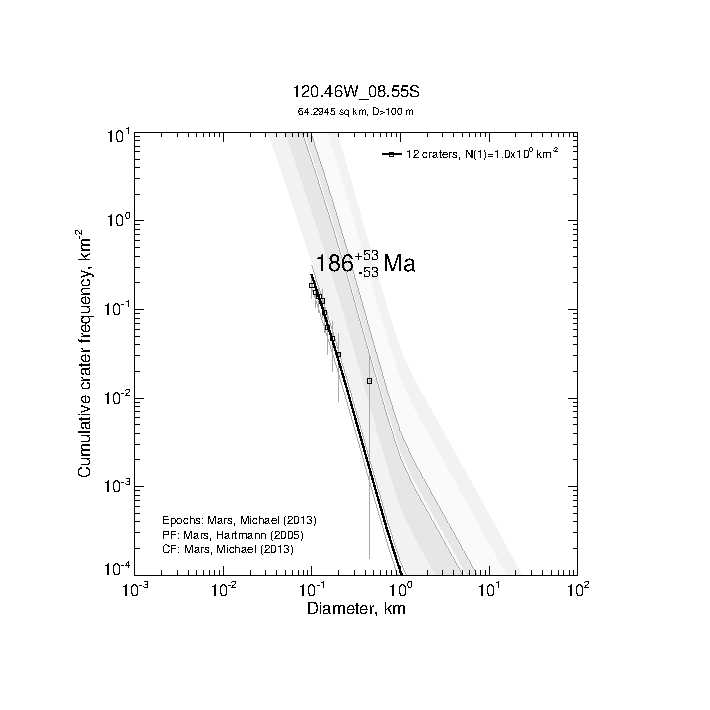
\includegraphics[width=\linewidth,clip,trim=1cm 1cm 1.5cm 1cm]{figures/craterstats/120-46W_08-55S_100m_cum.eps}
\end{subfigure}%
\begin{subfigure}{.33\textwidth}
  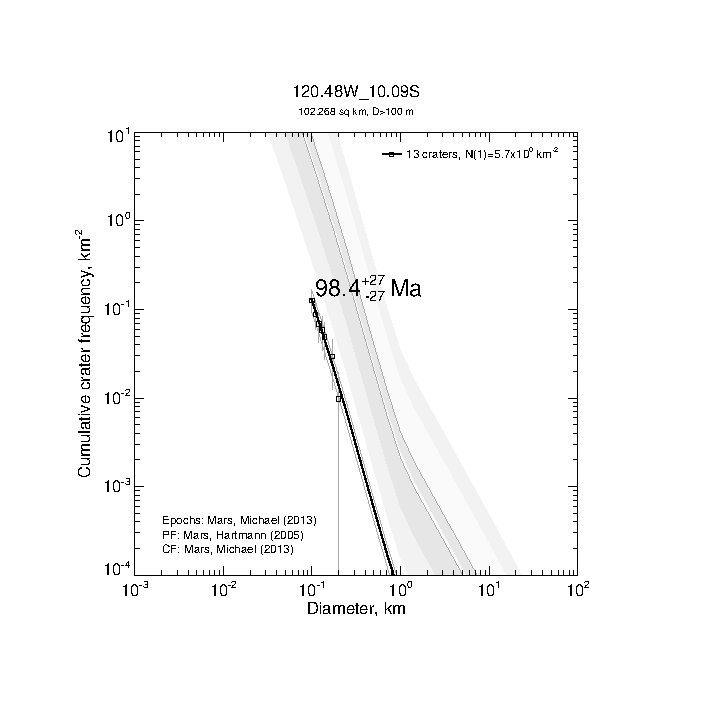
\includegraphics[width=\linewidth,clip,trim=1cm 1cm 1.5cm 1cm]{figures/craterstats/120-48W_10-09S_100m_cum.eps}
\end{subfigure}
\begin{subfigure}{.33\textwidth}
  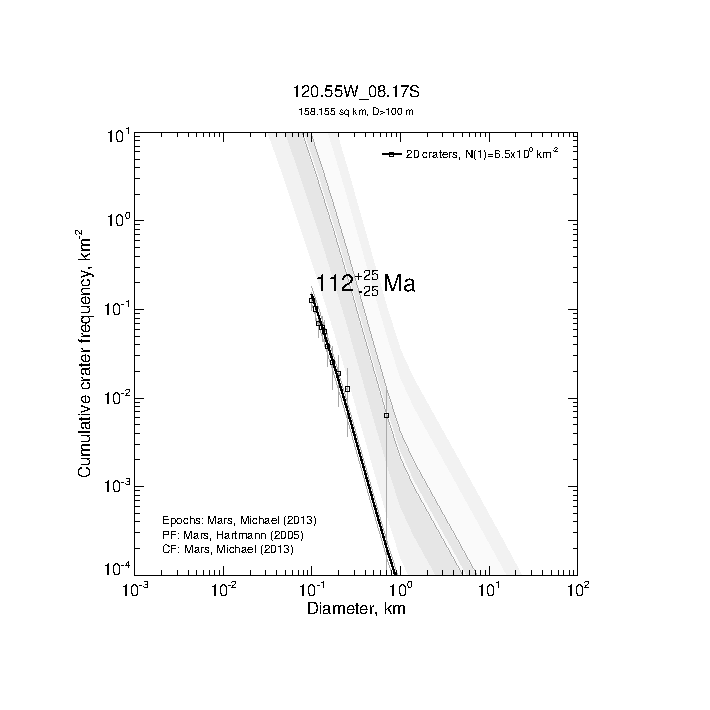
\includegraphics[width=\linewidth,clip,trim=1cm 1cm 1.5cm 1cm]{figures/craterstats/120-55W_08-17S_100m_cum.eps}
\end{subfigure}
\begin{subfigure}{.33\textwidth}
  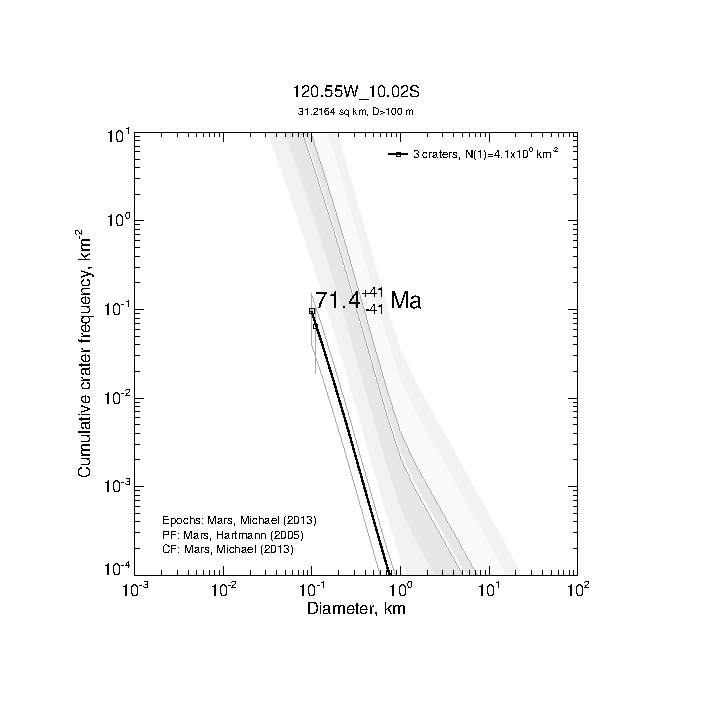
\includegraphics[width=\linewidth,clip,trim=1cm 1cm 1.5cm 1cm]{figures/craterstats/120-55W_10-02S_100m_cum.eps}
\end{subfigure}%
\begin{subfigure}{.33\textwidth}
  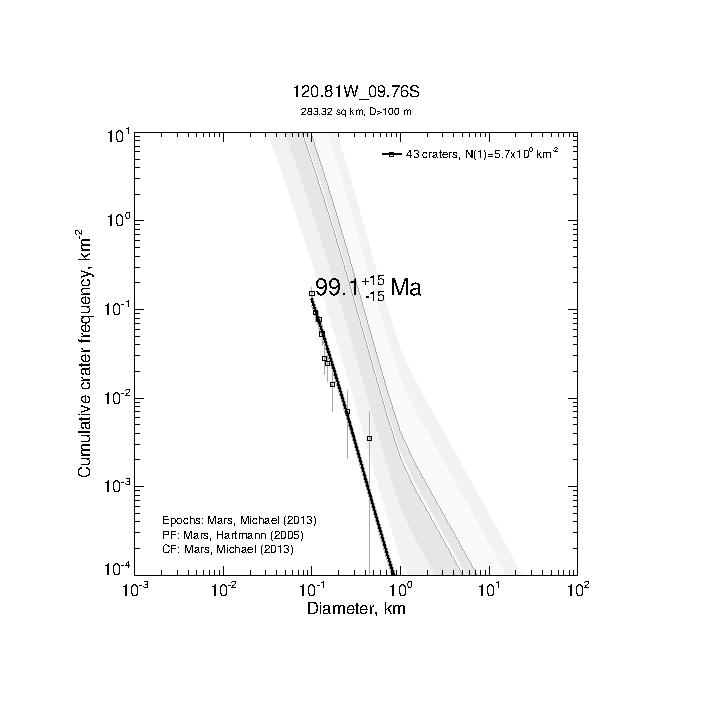
\includegraphics[width=\linewidth,clip,trim=1cm 1cm 1.5cm 1cm]{figures/craterstats/120-81W_09-76S_100m_cum.eps}
\end{subfigure}
\begin{subfigure}{.33\textwidth}
  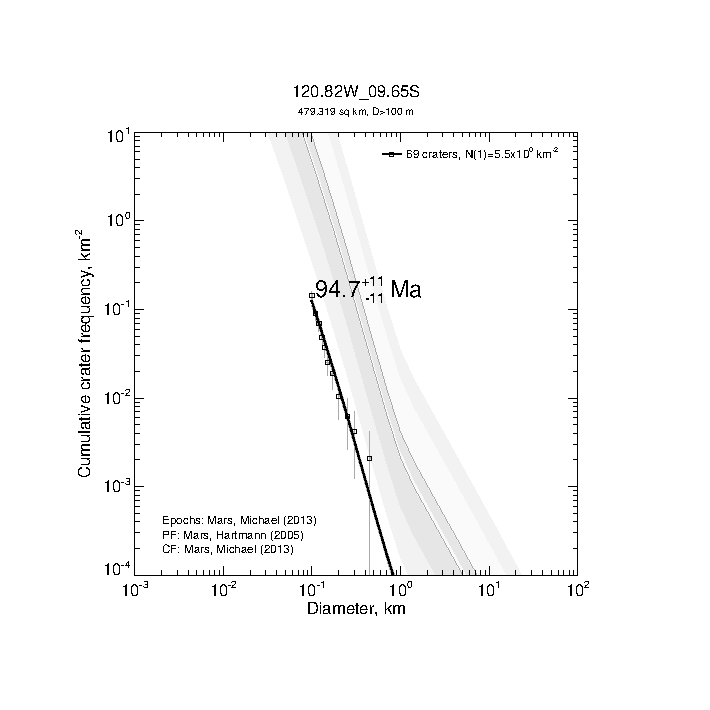
\includegraphics[width=\linewidth,clip,trim=1cm 1cm 1.5cm 1cm]{figures/craterstats/120-82W_09-65S_100m_cum.eps}
\end{subfigure}
\begin{subfigure}{.33\textwidth}
  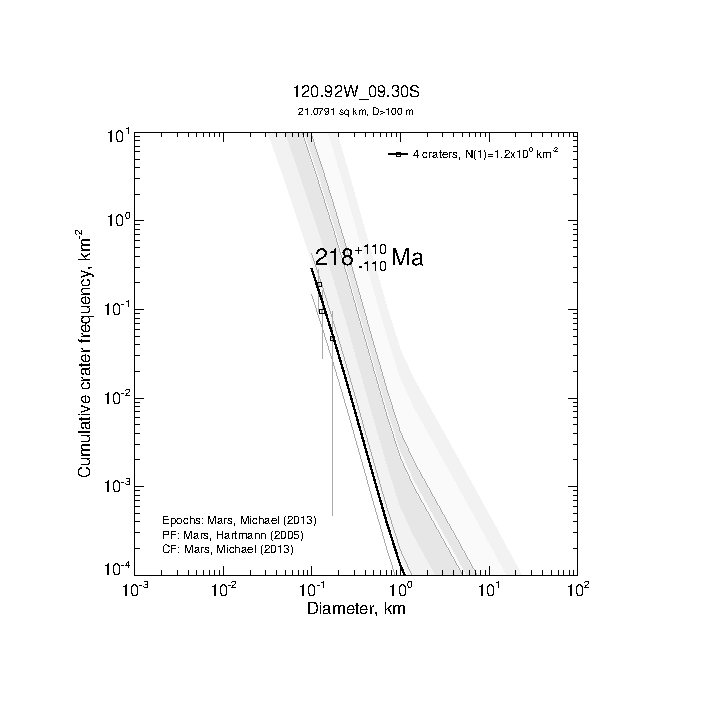
\includegraphics[width=\linewidth,clip,trim=1cm 1cm 1.5cm 1cm]{figures/craterstats/120-92W_09-30S_100m_cum.eps}
\end{subfigure}%
\begin{subfigure}{.33\textwidth}
  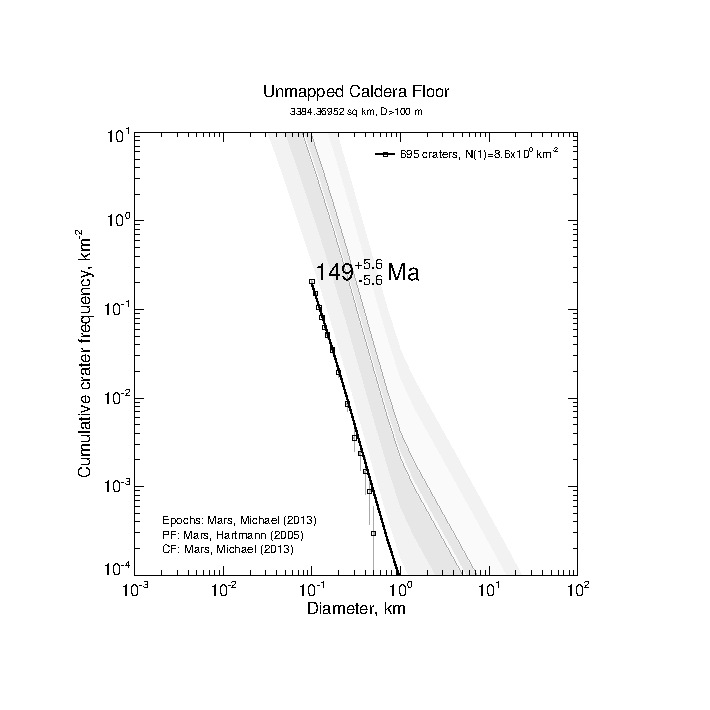
\includegraphics[width=\linewidth,clip,trim=1cm 1cm 1.5cm 1cm]{figures/craterstats/arsia_caldera_floor_100m_cum.eps}
\end{subfigure}
\begin{subfigure}{.33\textwidth}
  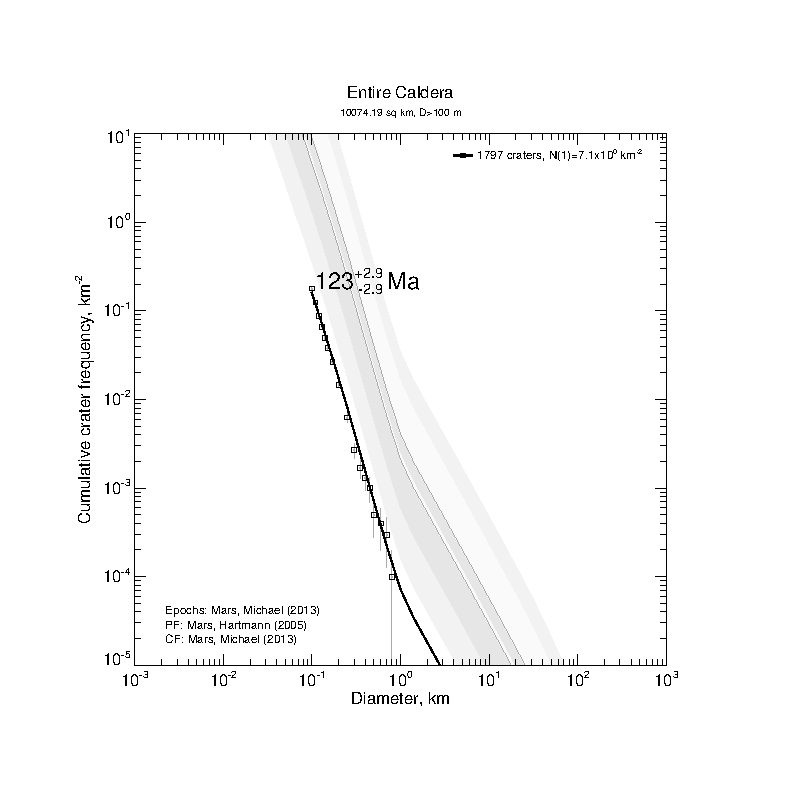
\includegraphics[width=\linewidth,clip,trim=1cm 1cm 1.5cm 1cm]{figures/craterstats/arsia_fullarea_100m_cum.eps}
\end{subfigure}
\end{figure}

\end{document}
